
\documentclass[a4paper,14pt]{extarticle}
\usepackage[left=1.2cm,right=1.2cm,top=1cm,bottom=2cm]{geometry}
\usepackage{fontspec}
\usepackage{polyglossia}
\setdefaultlanguage{russian}
\setotherlanguage{english}
\setmainfont{DejaVu Serif}
\setsansfont{DejaVu Sans}
\setmonofont{DejaVu Sans Mono}
\newfontfamily\cyrillicfont{DejaVu Serif}
\newfontfamily\cyrillicfontsf{DejaVu Sans}
\newfontfamily\cyrillicfonttt{DejaVu Sans Mono}
\usepackage{graphicx}
\usepackage{subcaption}
\usepackage{caption}
\usepackage{float}
\usepackage{array}
\usepackage{longtable}
\usepackage{booktabs}
\usepackage{hyperref}
\usepackage{xcolor}
\usepackage{multicol}
\setlength{\parindent}{0pt}
\linespread{1}
\captionsetup[table]{position=bottom}
\renewcommand{\arraystretch}{1.35}
\begin{document}
\begin{center}
МФТИ\\
\vspace{6cm}
{\large\textbf{Лабораторная работа 1}}\\[0.6cm]
{\Large\textbf{Обработка изображений}}\\[4cm]
{\large\textbf{Судаков Алексей}}\\[8cm]
Долгопрудный\\
2026
\end{center}
\pagebreak

\section*{Анализ гистограмм типов поверхности}
На исходном изображении выделены четыре типа поверхности и объектов: дорога, трава, поле и столбики в поле. Для каждого типа выбрано по 12 одинаковых блоков размером 18x18 пикселей. Для каждого блока рассчитаны средние значения каналов Red, Green, Blue и Gray. Канал Gray вычислялся по формуле $0{,}299R+0{,}587G+0{,}114B$.

\begin{figure}[H]
\centering
\begin{subfigure}[b]{0.19\textwidth}\centering
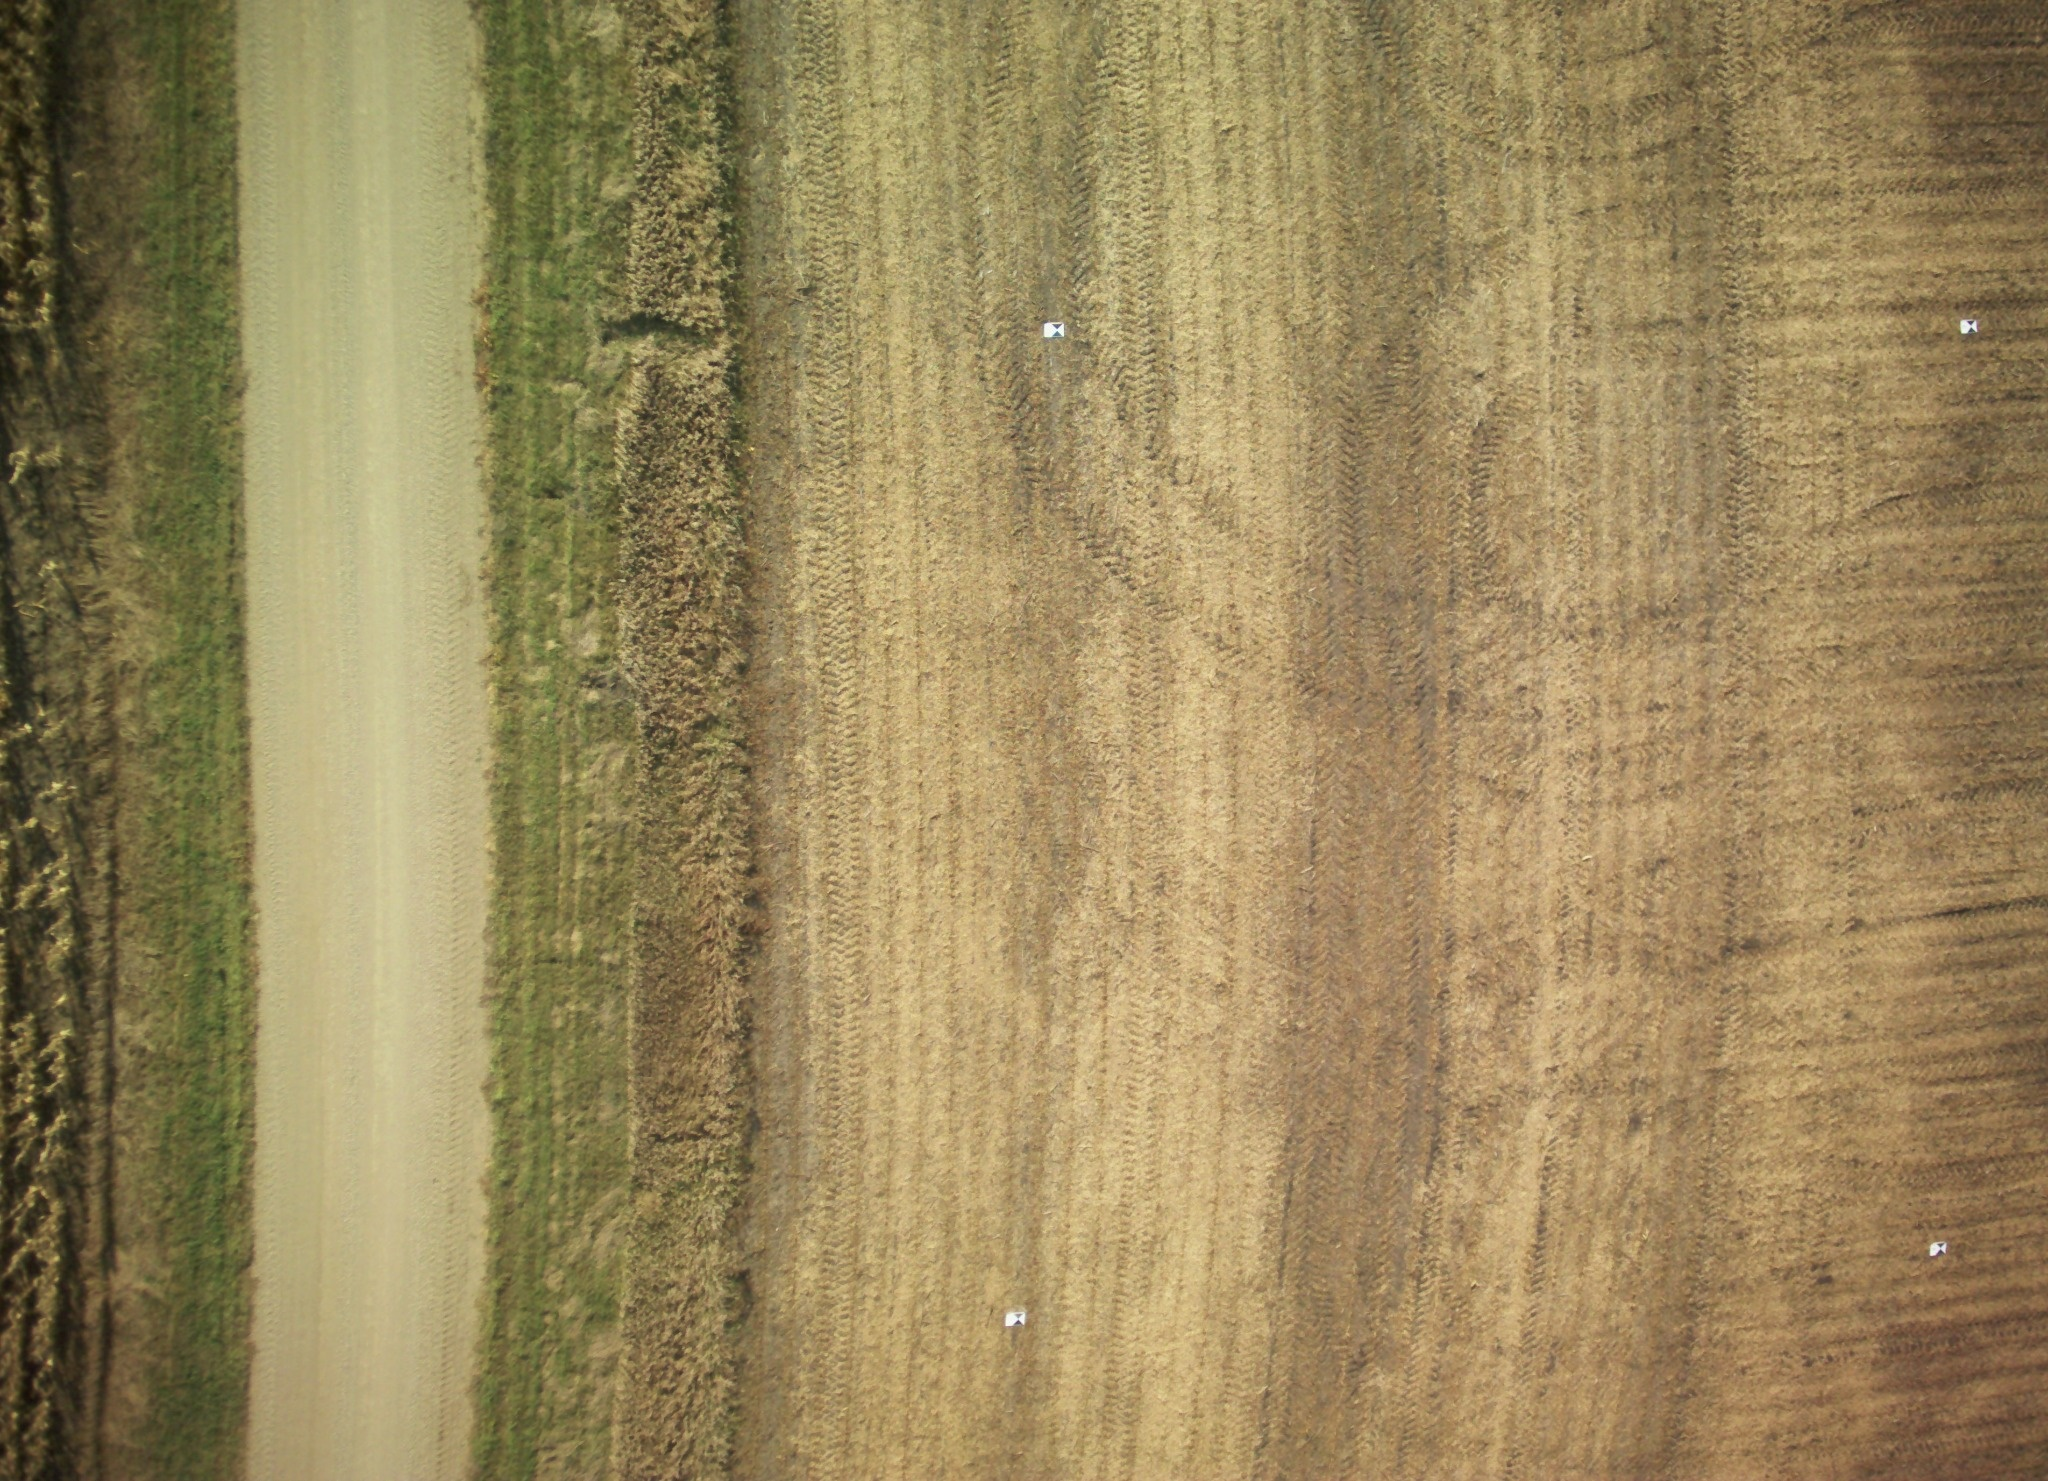
\includegraphics[width=\linewidth,height=5cm,keepaspectratio]{img/task_1/full_pic.jpg}
\caption{Целая картинка}
\end{subfigure}\hfill
\begin{subfigure}[b]{0.19\textwidth}\centering
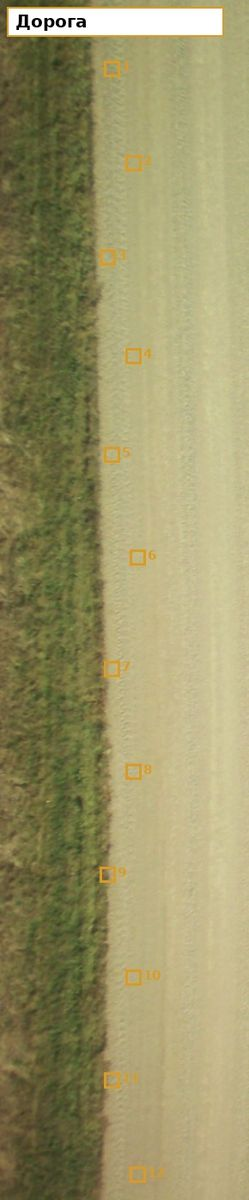
\includegraphics[width=\linewidth,height=5cm,keepaspectratio]{img/task_1/road.jpg}
\caption{Дорога}
\end{subfigure}\hfill
\begin{subfigure}[b]{0.19\textwidth}\centering
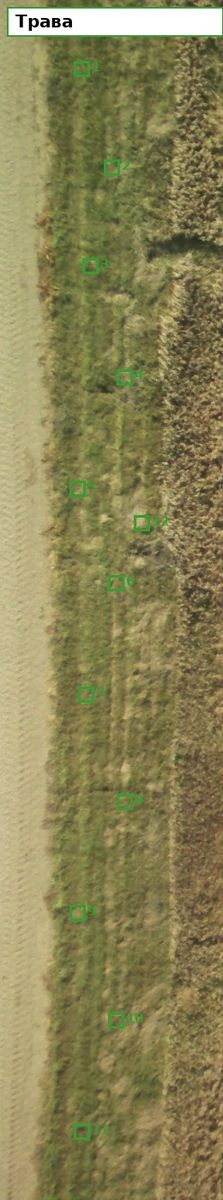
\includegraphics[width=\linewidth,height=5cm,keepaspectratio]{img/task_1/grass.jpg}
\caption{Трава}
\end{subfigure}\hfill
\begin{subfigure}[b]{0.19\textwidth}\centering
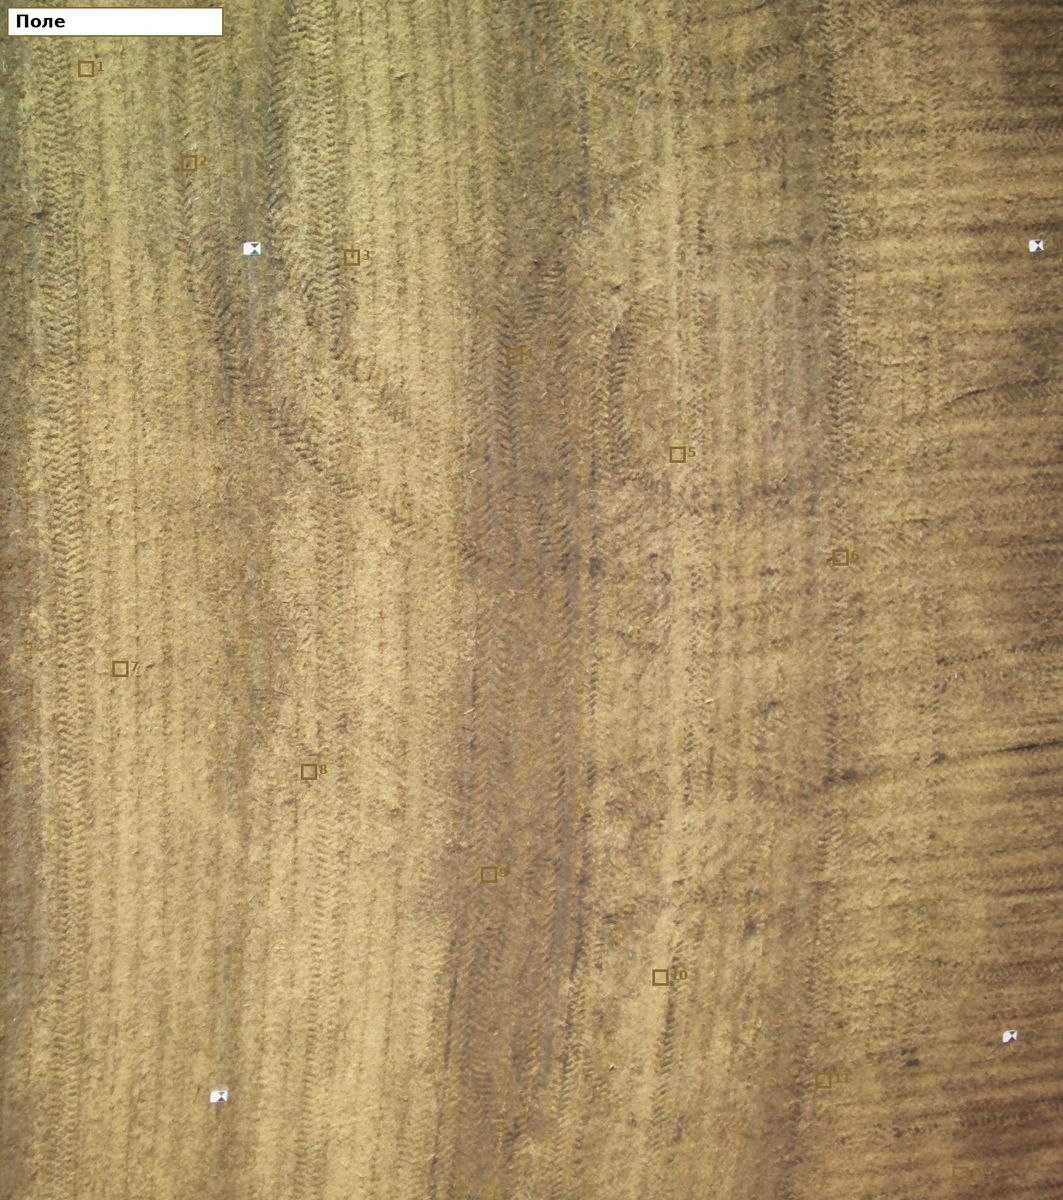
\includegraphics[width=\linewidth,height=5cm,keepaspectratio]{img/task_1/field.jpg}
\caption{Поле}
\end{subfigure}\hfill
\begin{subfigure}[b]{0.19\textwidth}\centering
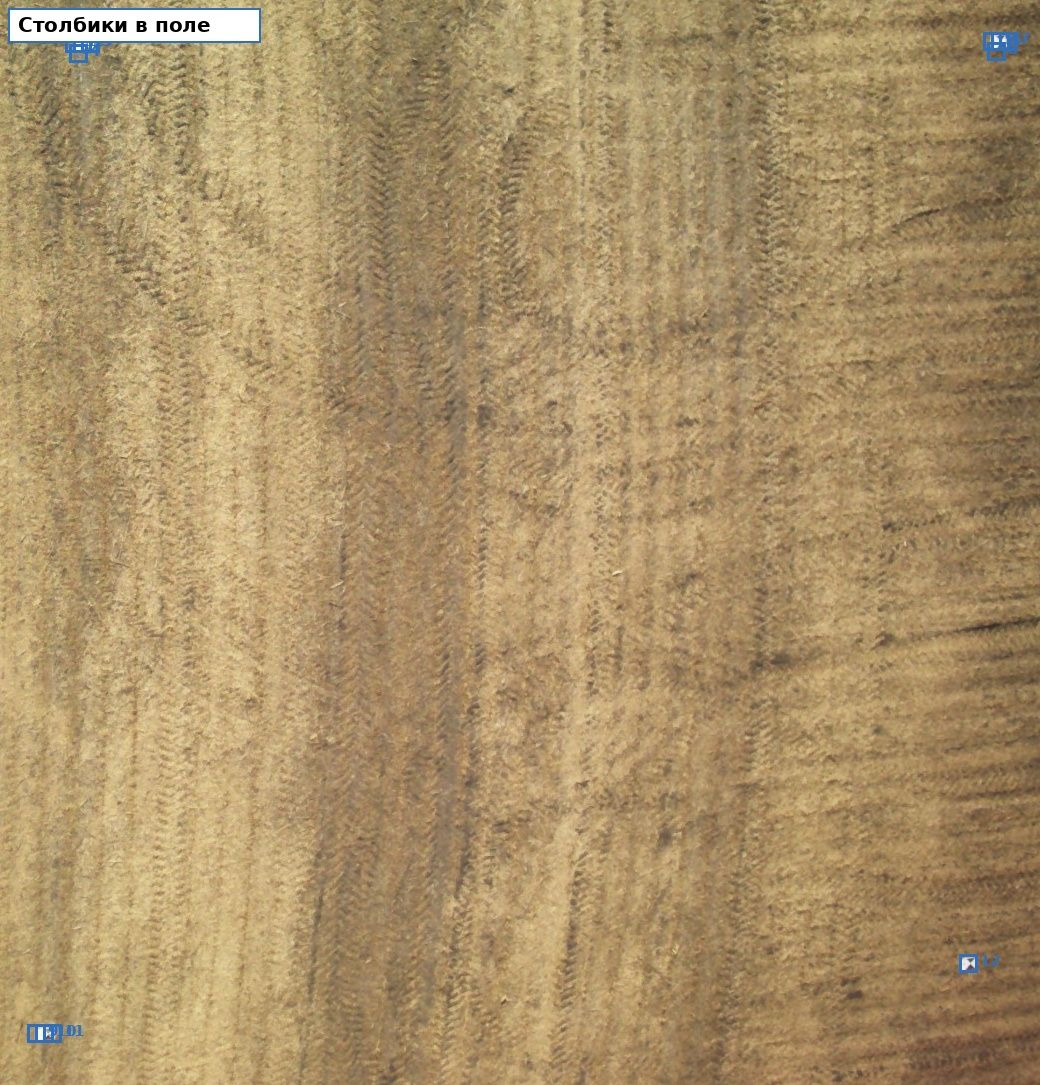
\includegraphics[width=\linewidth,height=5cm,keepaspectratio]{img/task_1/stakes.jpg}
\caption{Столбики в поле}
\end{subfigure}
\caption{Исходное изображение и выделенные области анализа}
\end{figure}

Средние значения интенсивности по всему изображению и по выделенным типам поверхности представлены в табл. 1.
\begin{table}[H]
\centering
\small
\begin{tabular}{|l|c|c|c|c|}
\hline
Тип поверхности & Red & Green & Blue & Gray \\\hline
Целое изображение & 152.84 & 135.29 & 93.17 & 135.74 \\ \hline
Дорога & 173.91 & 165.62 & 118.47 & 162.73 \\ \hline
Трава & 125.08 & 122.42 & 71.64 & 117.43 \\ \hline
Поле & 171.87 & 148.50 & 105.54 & 150.59 \\ \hline
Столбики в поле & 175.51 & 167.67 & 151.32 & 168.15 \\ \hline
\end{tabular}
\caption{Средние значения каналов}
\end{table}

\begin{figure}[H]\centering
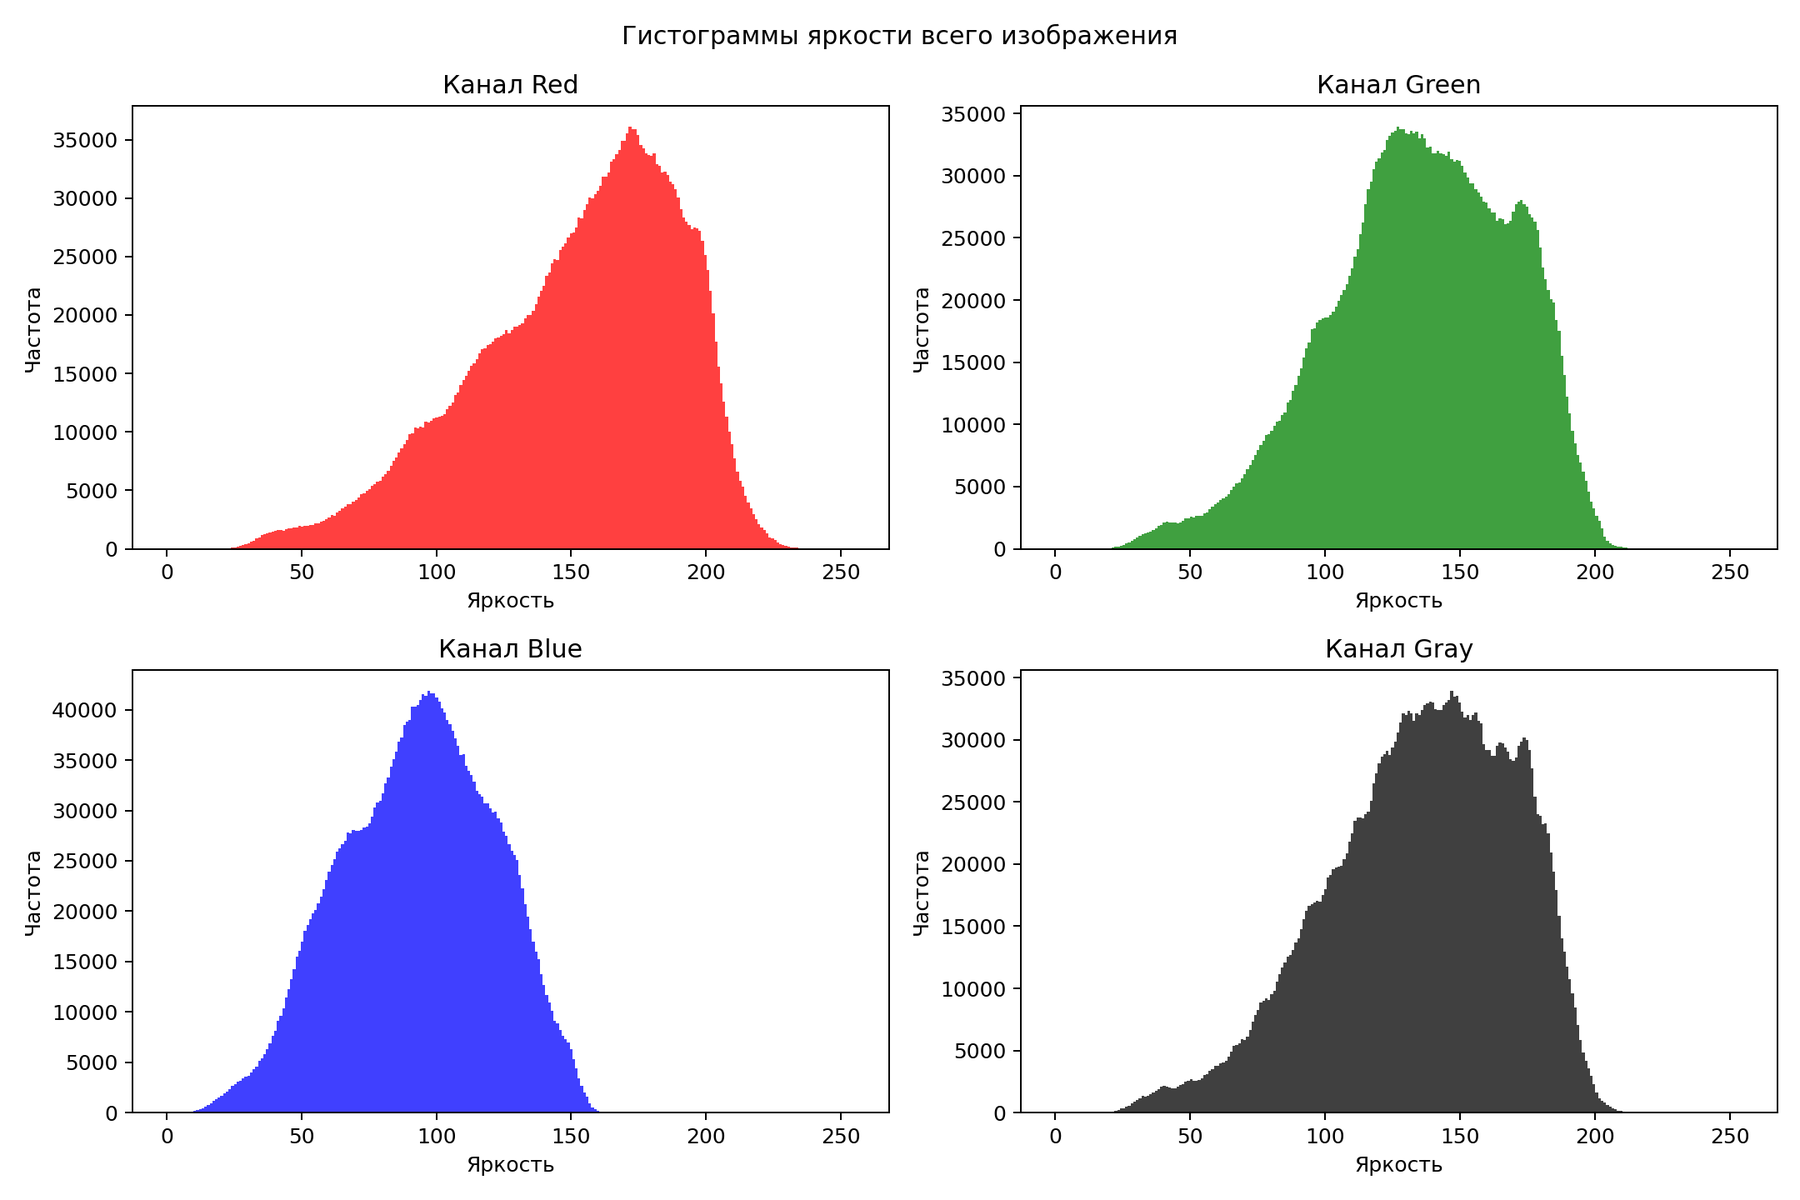
\includegraphics[width=0.92\textwidth]{img/histogram_whole_image.png}
\caption{Гистограммы яркости всего изображения}
\end{figure}

\begin{figure}[H]\centering
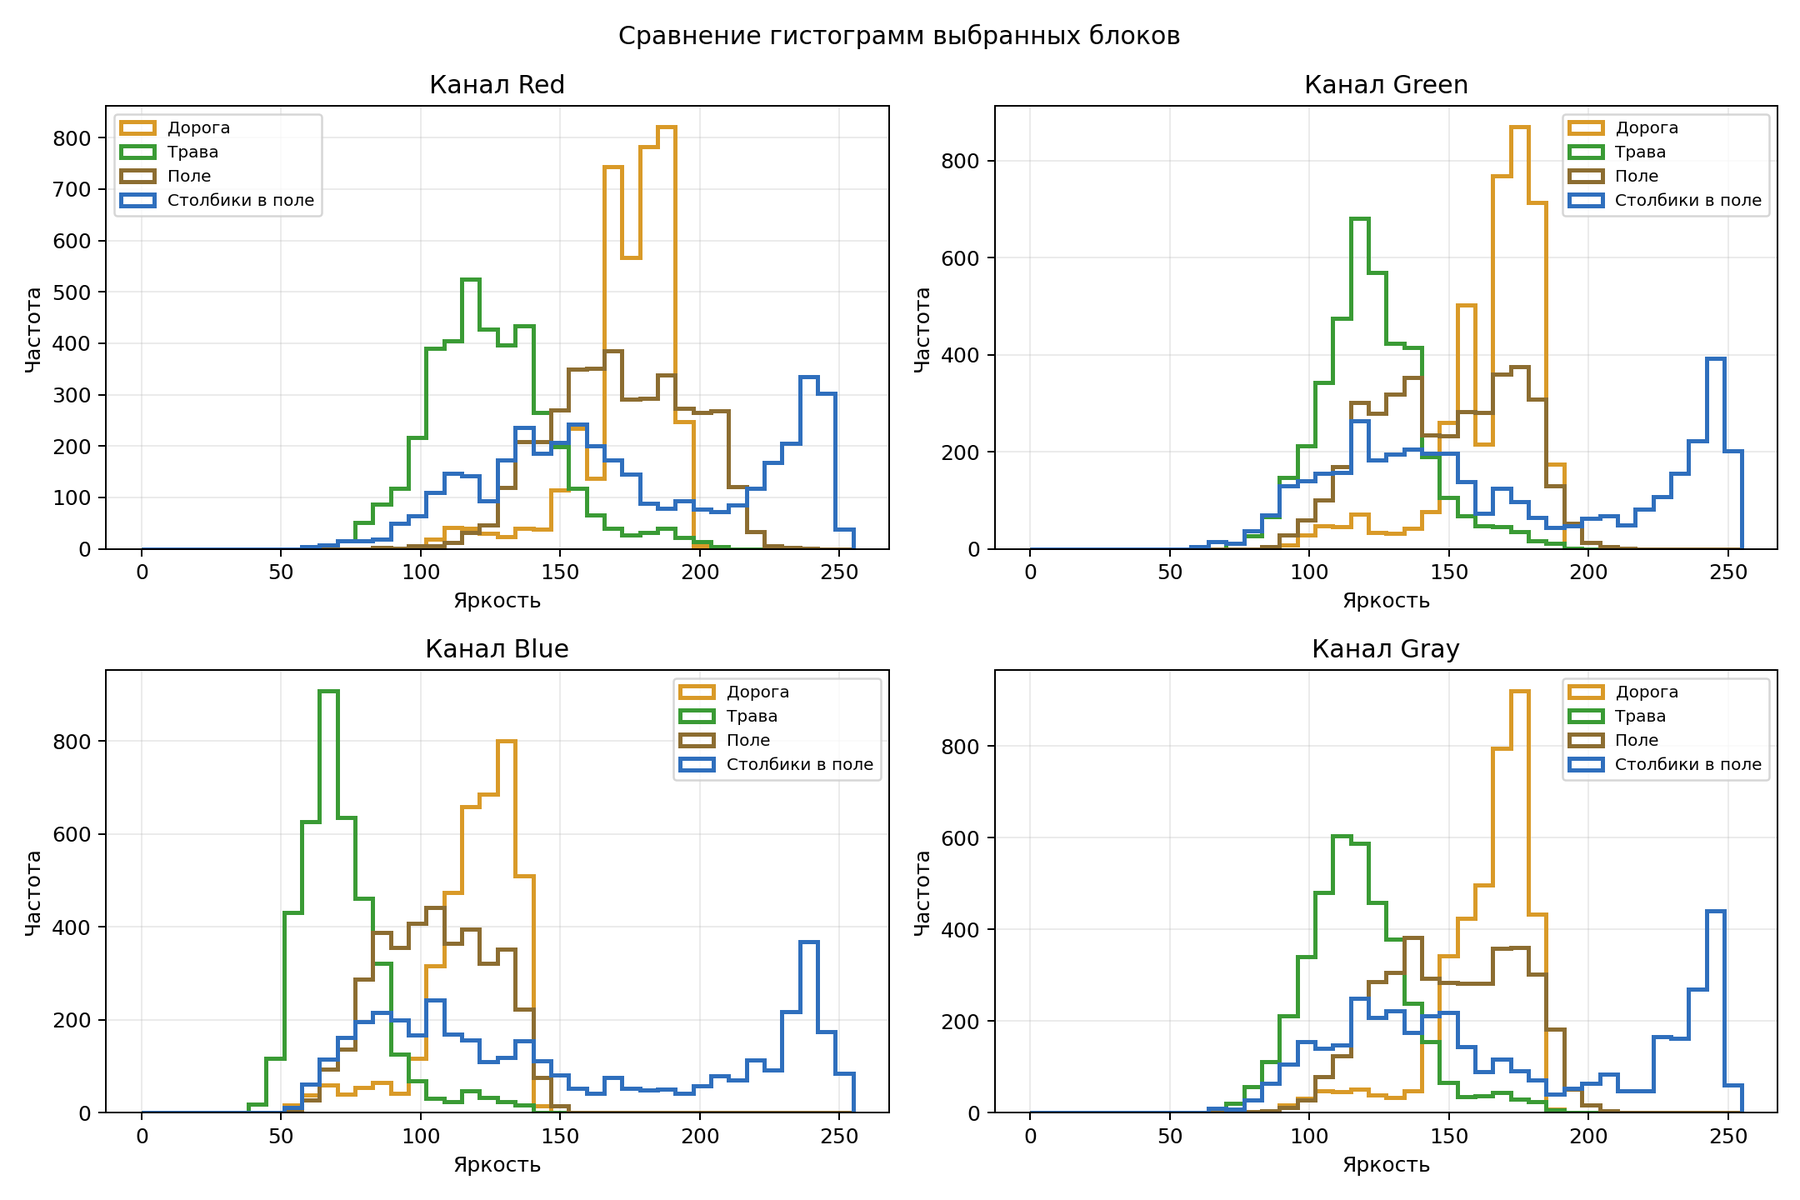
\includegraphics[width=0.92\textwidth]{img/histograms_selected_blocks.png}
\caption{Сравнение гистограмм выбранных блоков}
\end{figure}

\section*{Выделение блоков изображения}
Для измерений использовались блоки одинакового размера, чтобы сравнение средних значений не зависело от площади выбранного участка. Разметка блоков показана на рис. 4, а сами блоки в увеличенном виде - на рис. 5.

\begin{figure}[H]\centering
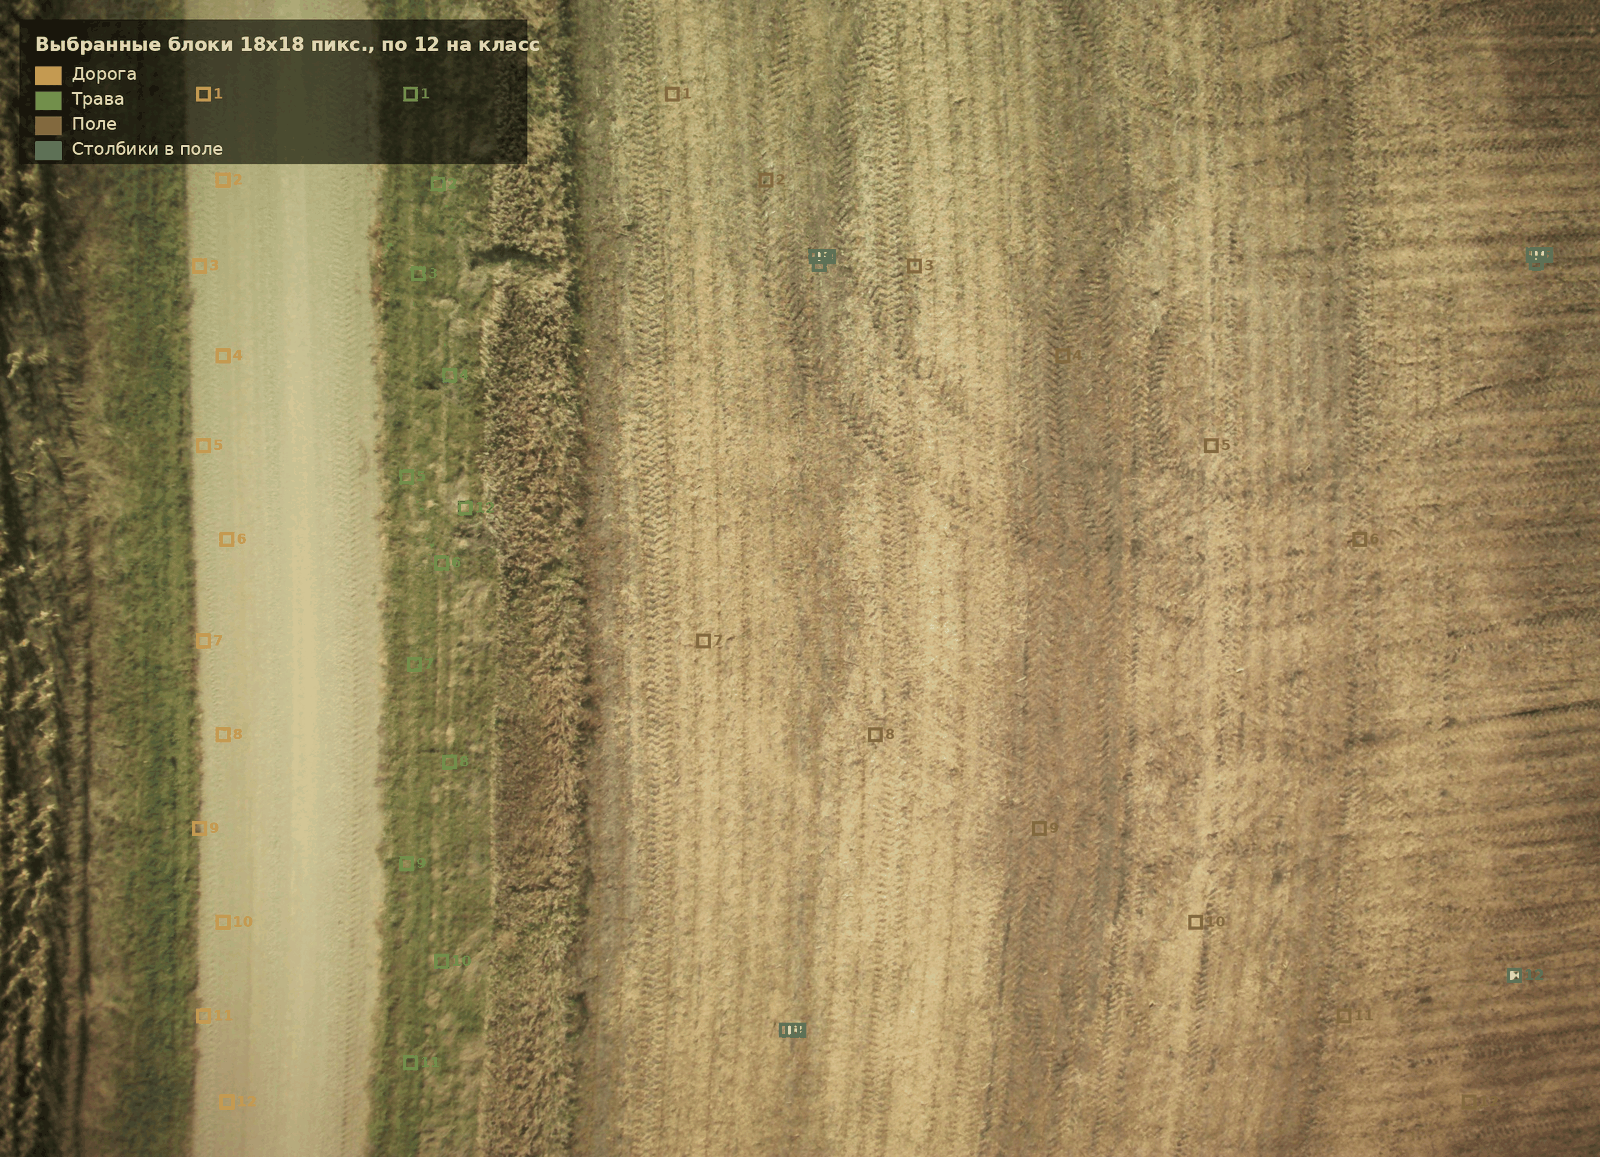
\includegraphics[width=0.92\textwidth]{img/selected_blocks_overview.png}
\caption{Выбранные блоки на исходном изображении}
\end{figure}

\begin{figure}[H]\centering
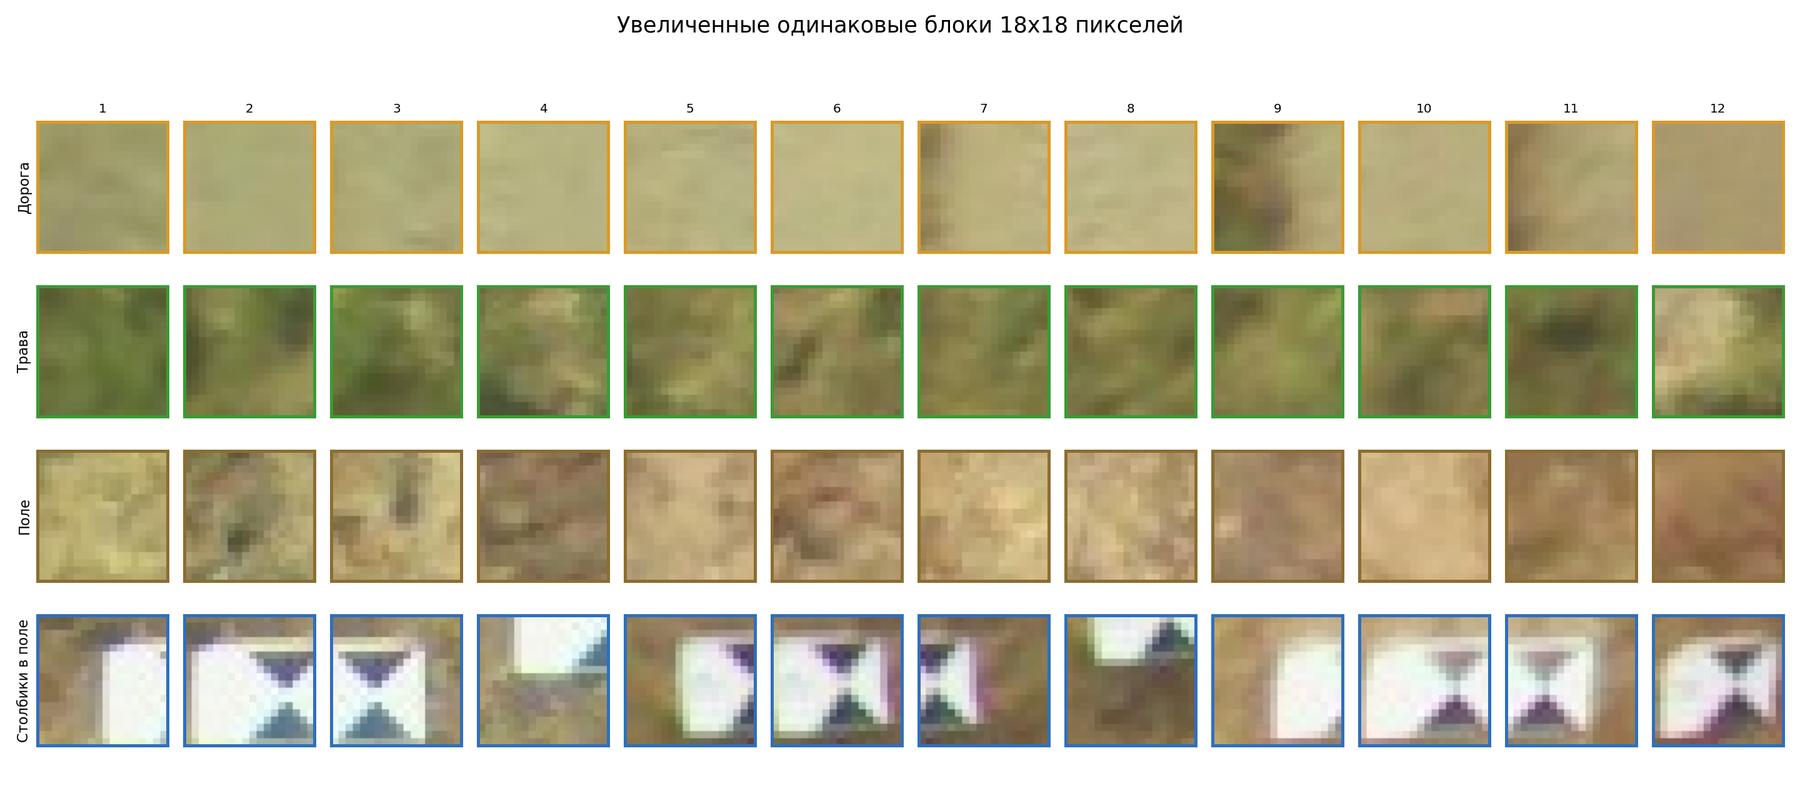
\includegraphics[width=0.98\textwidth]{img/sample_blocks_montage.png}
\caption{Увеличенные выбранные блоки}
\end{figure}

\section*{Статистический анализ: среднее и дисперсия}
В табл. 2 приведены координаты центров блоков и средние значения каналов. Полная таблица также сохранена в файлах measurements.xlsx и measurements.csv.

\begin{longtable}{|l|c|c|c|c|c|c|c|}
\hline
Тип & № & X & Y & Red & Green & Blue & Gray \\\hline
\endfirsthead
\hline
Тип & № & X & Y & Red & Green & Blue & Gray \\\hline
\endhead
Дорога & 1 & 260 & 120 & 155.90 & 153.27 & 105.00 & 148.56 \\ \hline
Дорога & 2 & 285 & 230 & 172.02 & 169.64 & 119.59 & 164.64 \\ \hline
Дорога & 3 & 255 & 340 & 172.19 & 169.13 & 119.75 & 164.41 \\ \hline
Дорога & 4 & 285 & 455 & 182.33 & 178.69 & 130.35 & 174.27 \\ \hline
Дорога & 5 & 260 & 570 & 181.43 & 175.76 & 127.06 & 171.90 \\ \hline
Дорога & 6 & 290 & 690 & 190.18 & 183.63 & 135.25 & 180.07 \\ \hline
Дорога & 7 & 260 & 820 & 179.58 & 167.47 & 118.66 & 165.53 \\ \hline
Дорога & 8 & 285 & 940 & 189.24 & 180.46 & 134.31 & 177.82 \\ \hline
Дорога & 9 & 255 & 1060 & 144.47 & 132.71 & 88.76 & 131.21 \\ \hline
Дорога & 10 & 285 & 1180 & 183.83 & 173.65 & 126.61 & 171.33 \\ \hline
Дорога & 11 & 260 & 1300 & 165.49 & 149.82 & 105.43 & 149.44 \\ \hline
Дорога & 12 & 290 & 1410 & 170.26 & 153.26 & 110.87 & 153.51 \\ \hline
Трава & 1 & 525 & 120 & 103.20 & 112.91 & 59.25 & 103.89 \\ \hline
Трава & 2 & 560 & 235 & 116.98 & 118.12 & 67.60 & 112.02 \\ \hline
Трава & 3 & 535 & 350 & 110.84 & 116.84 & 63.93 & 109.02 \\ \hline
Трава & 4 & 575 & 480 & 127.58 & 127.19 & 78.35 & 121.74 \\ \hline
Трава & 5 & 520 & 610 & 131.47 & 127.94 & 74.69 & 122.92 \\ \hline
Трава & 6 & 565 & 720 & 133.61 & 124.96 & 76.84 & 122.06 \\ \hline
Трава & 7 & 530 & 850 & 128.94 & 124.09 & 71.03 & 119.49 \\ \hline
Трава & 8 & 575 & 975 & 124.95 & 118.95 & 67.44 & 114.87 \\ \hline
Трава & 9 & 520 & 1105 & 132.35 & 128.96 & 72.71 & 123.56 \\ \hline
Трава & 10 & 565 & 1230 & 128.29 & 119.33 & 71.96 & 116.61 \\ \hline
Трава & 11 & 525 & 1360 & 107.47 & 103.66 & 59.81 & 99.80 \\ \hline
Трава & 12 & 595 & 650 & 155.28 & 146.10 & 96.09 & 143.15 \\ \hline
Поле & 1 & 860 & 120 & 181.10 & 169.48 & 109.98 & 166.17 \\ \hline
Поле & 2 & 980 & 230 & 150.90 & 140.38 & 97.88 & 138.68 \\ \hline
Поле & 3 & 1170 & 340 & 176.75 & 160.13 & 112.09 & 159.62 \\ \hline
Поле & 4 & 1360 & 455 & 139.25 & 119.51 & 87.44 & 121.76 \\ \hline
Поле & 5 & 1550 & 570 & 188.67 & 165.08 & 122.72 & 167.30 \\ \hline
Поле & 6 & 1740 & 690 & 164.11 & 136.82 & 99.45 & 140.72 \\ \hline
Поле & 7 & 900 & 820 & 196.64 & 171.87 & 121.22 & 173.50 \\ \hline
Поле & 8 & 1120 & 940 & 188.72 & 164.02 & 121.05 & 166.51 \\ \hline
Поле & 9 & 1330 & 1060 & 162.90 & 134.93 & 101.50 & 139.48 \\ \hline
Поле & 10 & 1530 & 1180 & 204.31 & 175.09 & 127.66 & 178.42 \\ \hline
Поле & 11 & 1720 & 1300 & 156.74 & 127.70 & 85.65 & 131.59 \\ \hline
Поле & 12 & 1880 & 1410 & 152.41 & 116.97 & 79.88 & 123.34 \\ \hline
Столбики в поле & 1 & 1044 & 328 & 181.52 & 174.09 & 154.78 & 174.11 \\ \hline
Столбики в поле & 2 & 1052 & 328 & 191.38 & 193.75 & 187.73 & 192.35 \\ \hline
Столбики в поле & 3 & 1060 & 328 & 177.84 & 177.86 & 165.50 & 176.44 \\ \hline
Столбики в поле & 4 & 1048 & 338 & 174.26 & 171.65 & 149.37 & 169.89 \\ \hline
Столбики в поле & 5 & 1962 & 326 & 166.49 & 157.96 & 136.62 & 158.08 \\ \hline
Столбики в поле & 6 & 1970 & 326 & 170.68 & 165.45 & 158.56 & 166.23 \\ \hline
Столбики в поле & 7 & 1978 & 326 & 140.05 & 126.31 & 109.43 & 128.50 \\ \hline
Столбики в поле & 8 & 1966 & 336 & 136.37 & 127.25 & 103.16 & 127.23 \\ \hline
Столбики в поле & 9 & 1006 & 1318 & 200.25 & 184.92 & 158.06 & 186.44 \\ \hline
Столбики в поле & 10 & 1014 & 1318 & 206.31 & 199.17 & 187.06 & 199.92 \\ \hline
Столбики в поле & 11 & 1022 & 1318 & 184.67 & 172.21 & 155.11 & 173.99 \\ \hline
Столбики в поле & 12 & 1938 & 1248 & 176.30 & 161.36 & 150.46 & 164.59 \\ \hline
\caption{Интенсивности выбранных участков изображения}
\end{longtable}

\begin{table}[H]
\centering
\scriptsize
\begin{tabular}{|l|c|c|c|c|c|c|c|c|c|c|}
\hline
Тип & N & R ср. & R дисп. & G ср. & G дисп. & B ср. & B дисп. & Gray ср. & Gray дисп. \\\hline
Целое изображение & - & 152.84 & - & 135.29 & - & 93.17 & - & 135.74 & - \\ \hline
Дорога & 12 & 173.91 & 185.39 & 165.62 & 232.03 & 118.47 & 191.69 & 162.73 & 208.14 \\ \hline
Трава & 12 & 125.08 & 197.03 & 122.42 & 107.24 & 71.64 & 97.04 & 117.43 & 124.98 \\ \hline
Поле & 12 & 171.87 & 417.56 & 148.50 & 454.32 & 105.54 & 257.00 & 150.59 & 404.90 \\ \hline
Столбики в поле & 12 & 175.51 & 439.44 & 167.67 & 512.22 & 151.32 & 656.74 & 168.15 & 494.18 \\ \hline
\end{tabular}
\caption{Средние значения и дисперсии по каждому типу поверхности}
\end{table}

\begin{figure}[H]
\centering
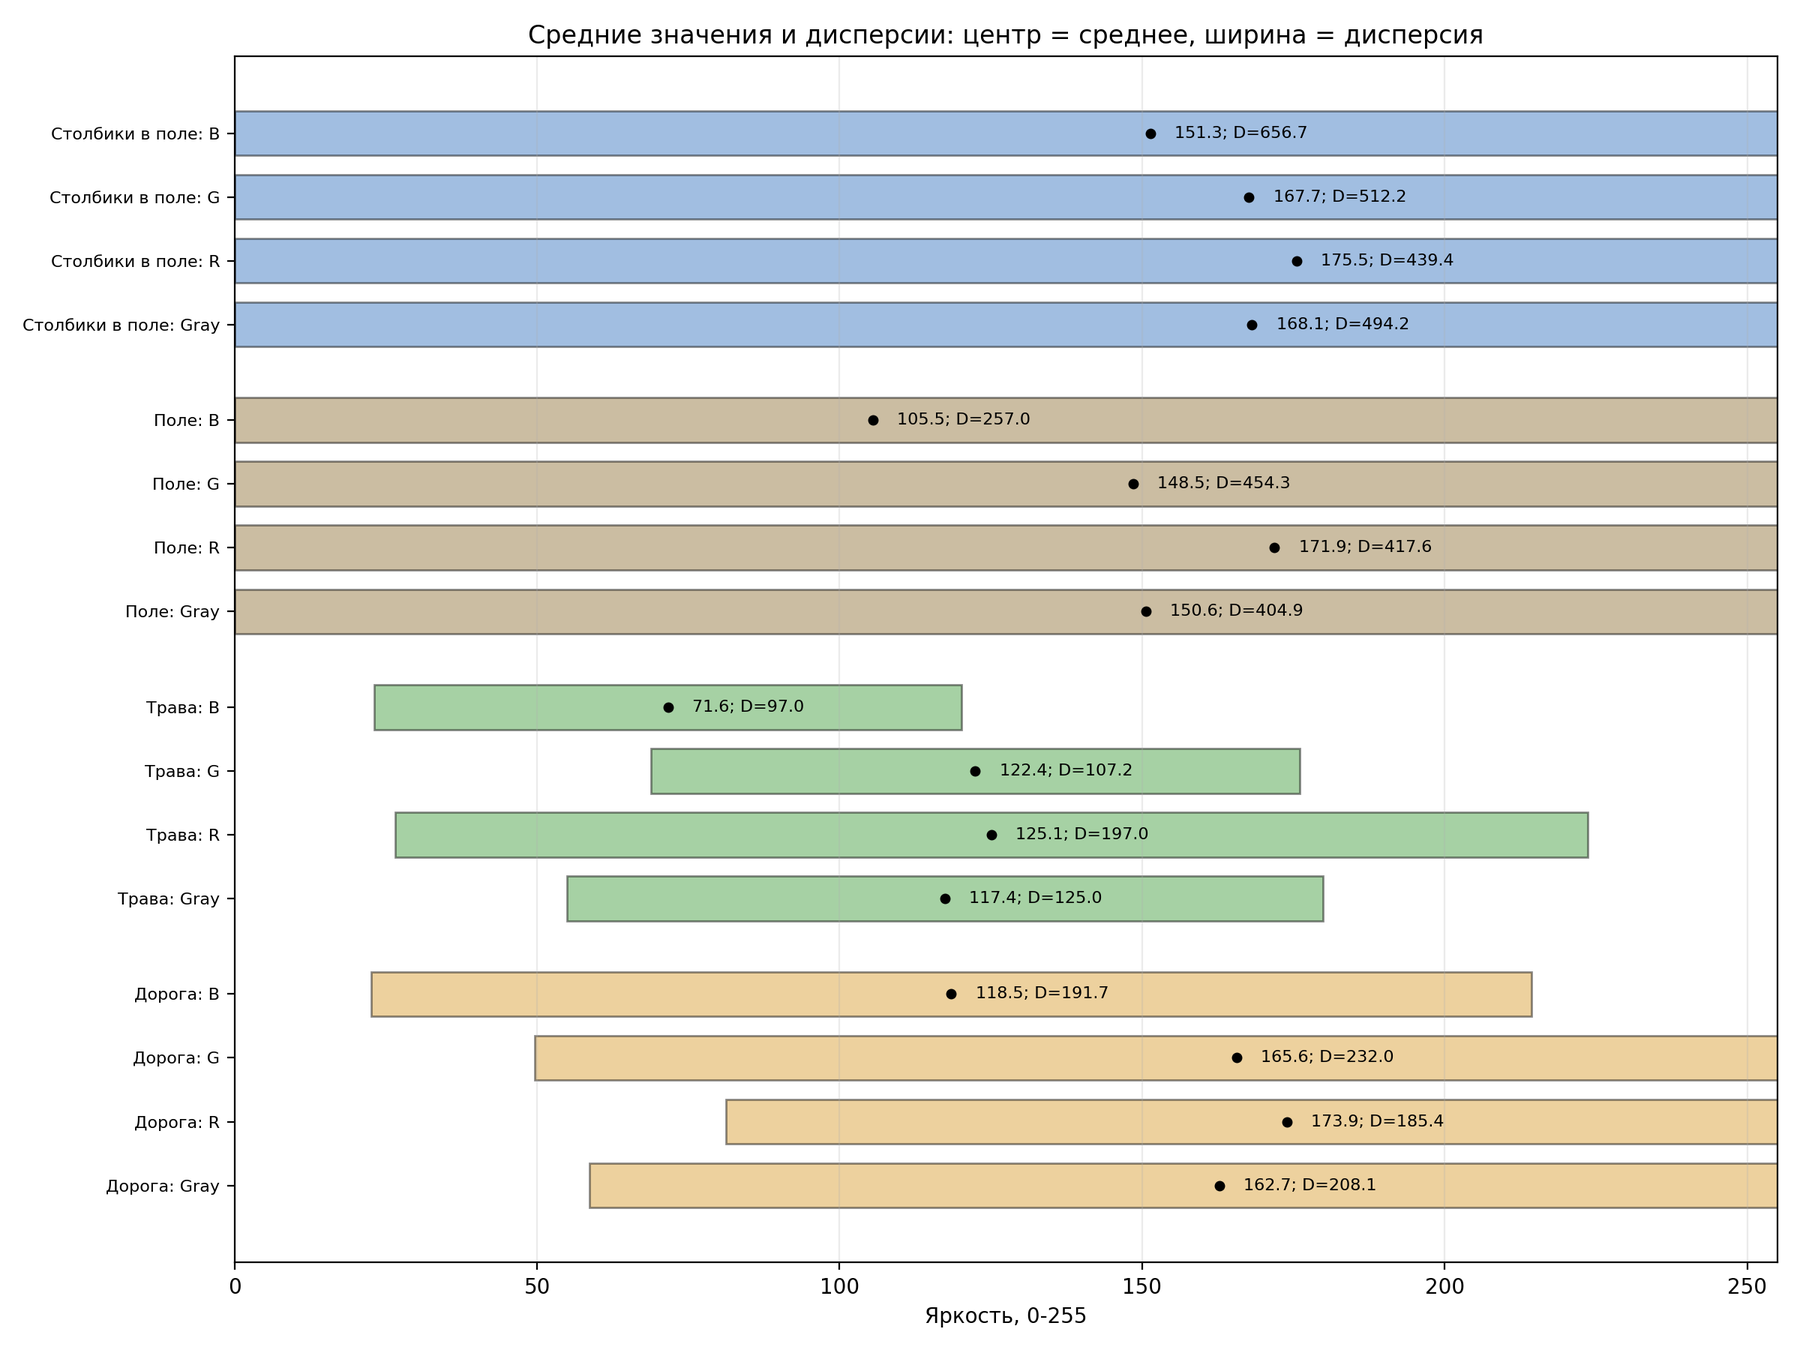
\includegraphics[width=0.92\textwidth]{img/mean_and_error.png}
\caption{Средние значения и дисперсии: центр прямоугольника - среднее, ширина - дисперсия}
\end{figure}

\begin{figure}[H]
\centering
\begin{subfigure}[b]{0.49\textwidth}\centering
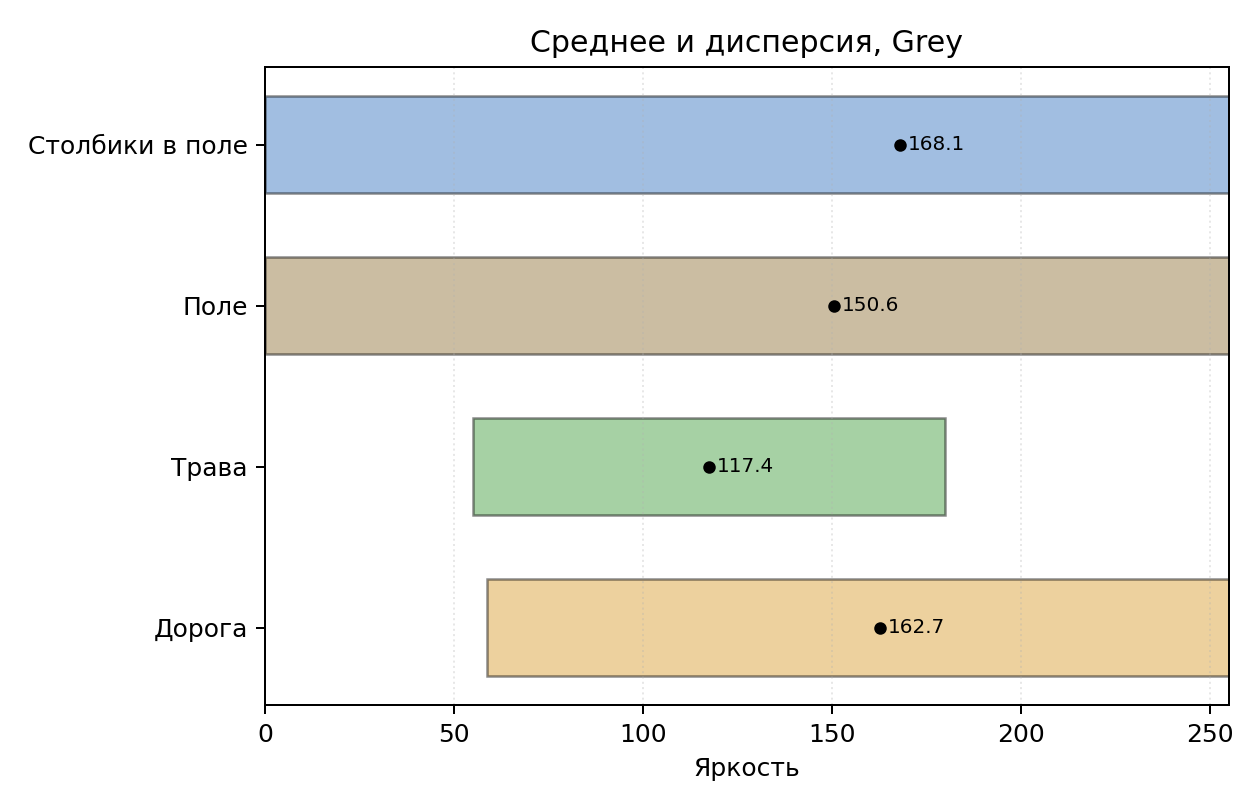
\includegraphics[width=\linewidth]{img/mean_and_error_Grey.png}
\caption{Grey}
\end{subfigure}\hfill
\begin{subfigure}[b]{0.49\textwidth}\centering
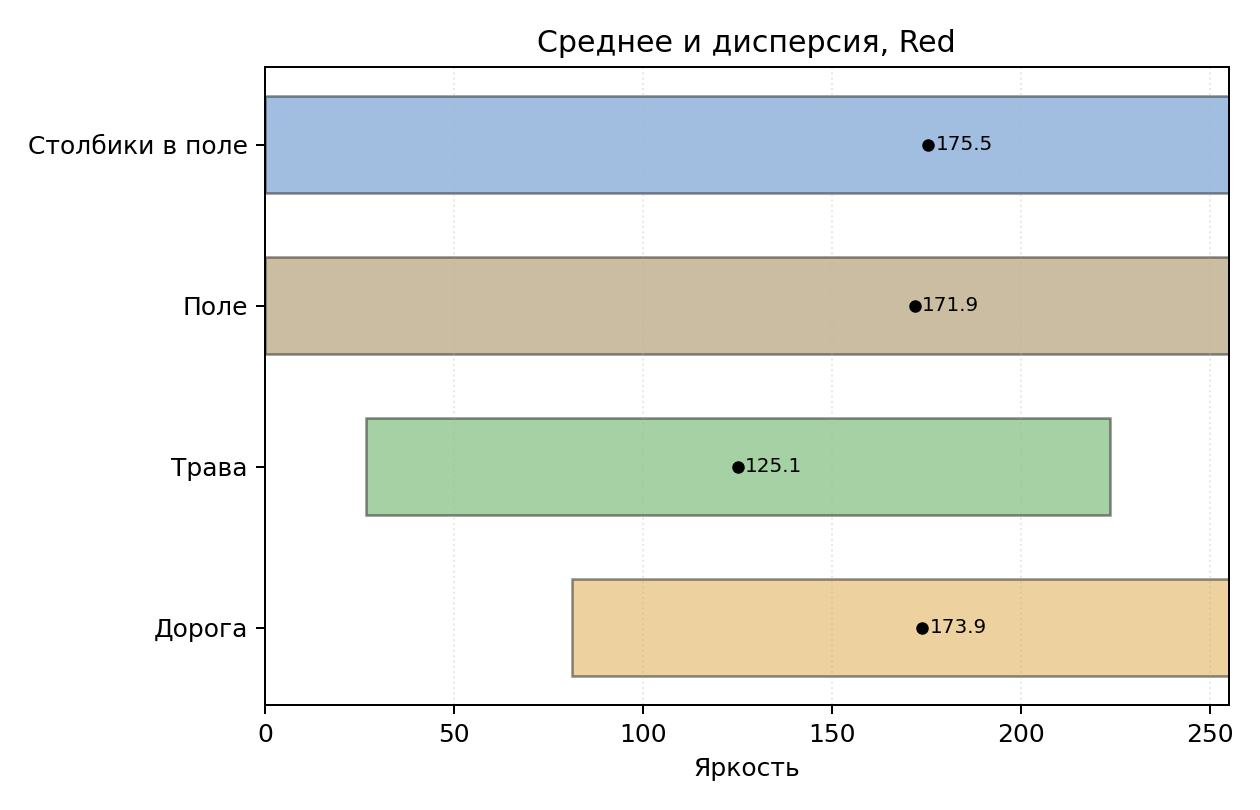
\includegraphics[width=\linewidth]{img/mean_and_error_Red.png}
\caption{Red}
\end{subfigure}\\[0.3cm]
\begin{subfigure}[b]{0.49\textwidth}\centering
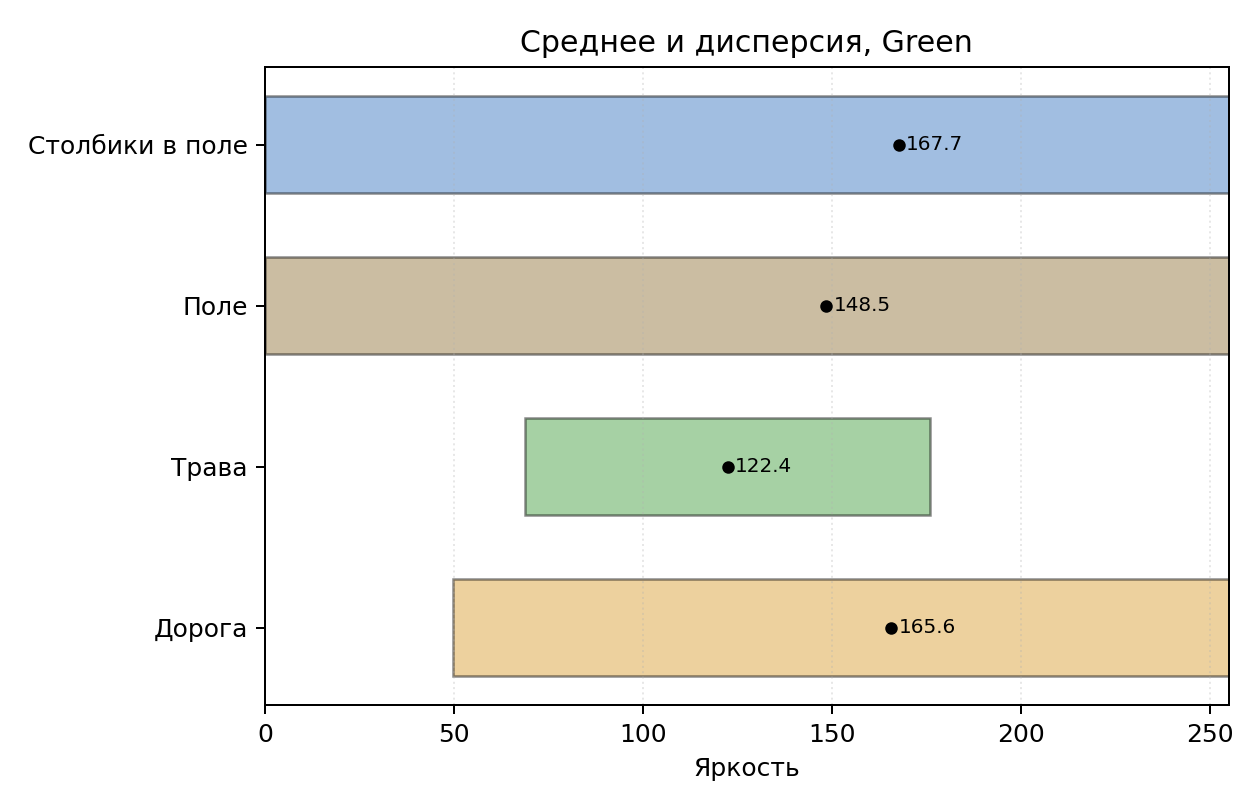
\includegraphics[width=\linewidth]{img/mean_and_error_Green.png}
\caption{Green}
\end{subfigure}\hfill
\begin{subfigure}[b]{0.49\textwidth}\centering
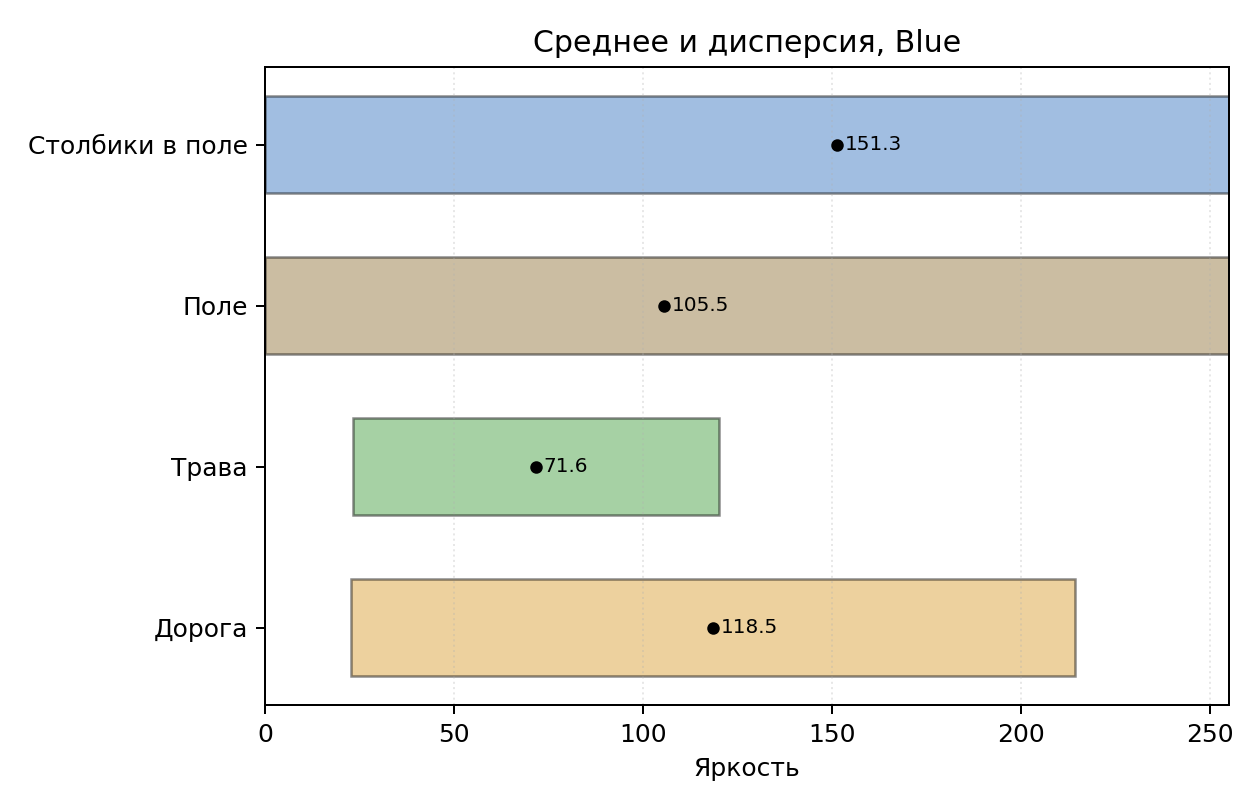
\includegraphics[width=\linewidth]{img/mean_and_error_Blue.png}
\caption{Blue}
\end{subfigure}
\caption{Средние значения и дисперсии по отдельным каналам}
\end{figure}

\section*{Анализ разделения типов поверхности в RGB}
Дорога и поле имеют близкие значения красного канала, но различаются по зеленому и синему каналам, а также по величине дисперсии. Трава отделяется от остальных типов поверхностей более низким значением Blue. Столбики в поле имеют повышенные Gray и Blue, поэтому на RGB-графиках они отделяются от фона поля лучше, чем участки дороги и поля между собой.

\begin{figure}[H]
\centering
\begin{subfigure}[b]{0.49\textwidth}\centering
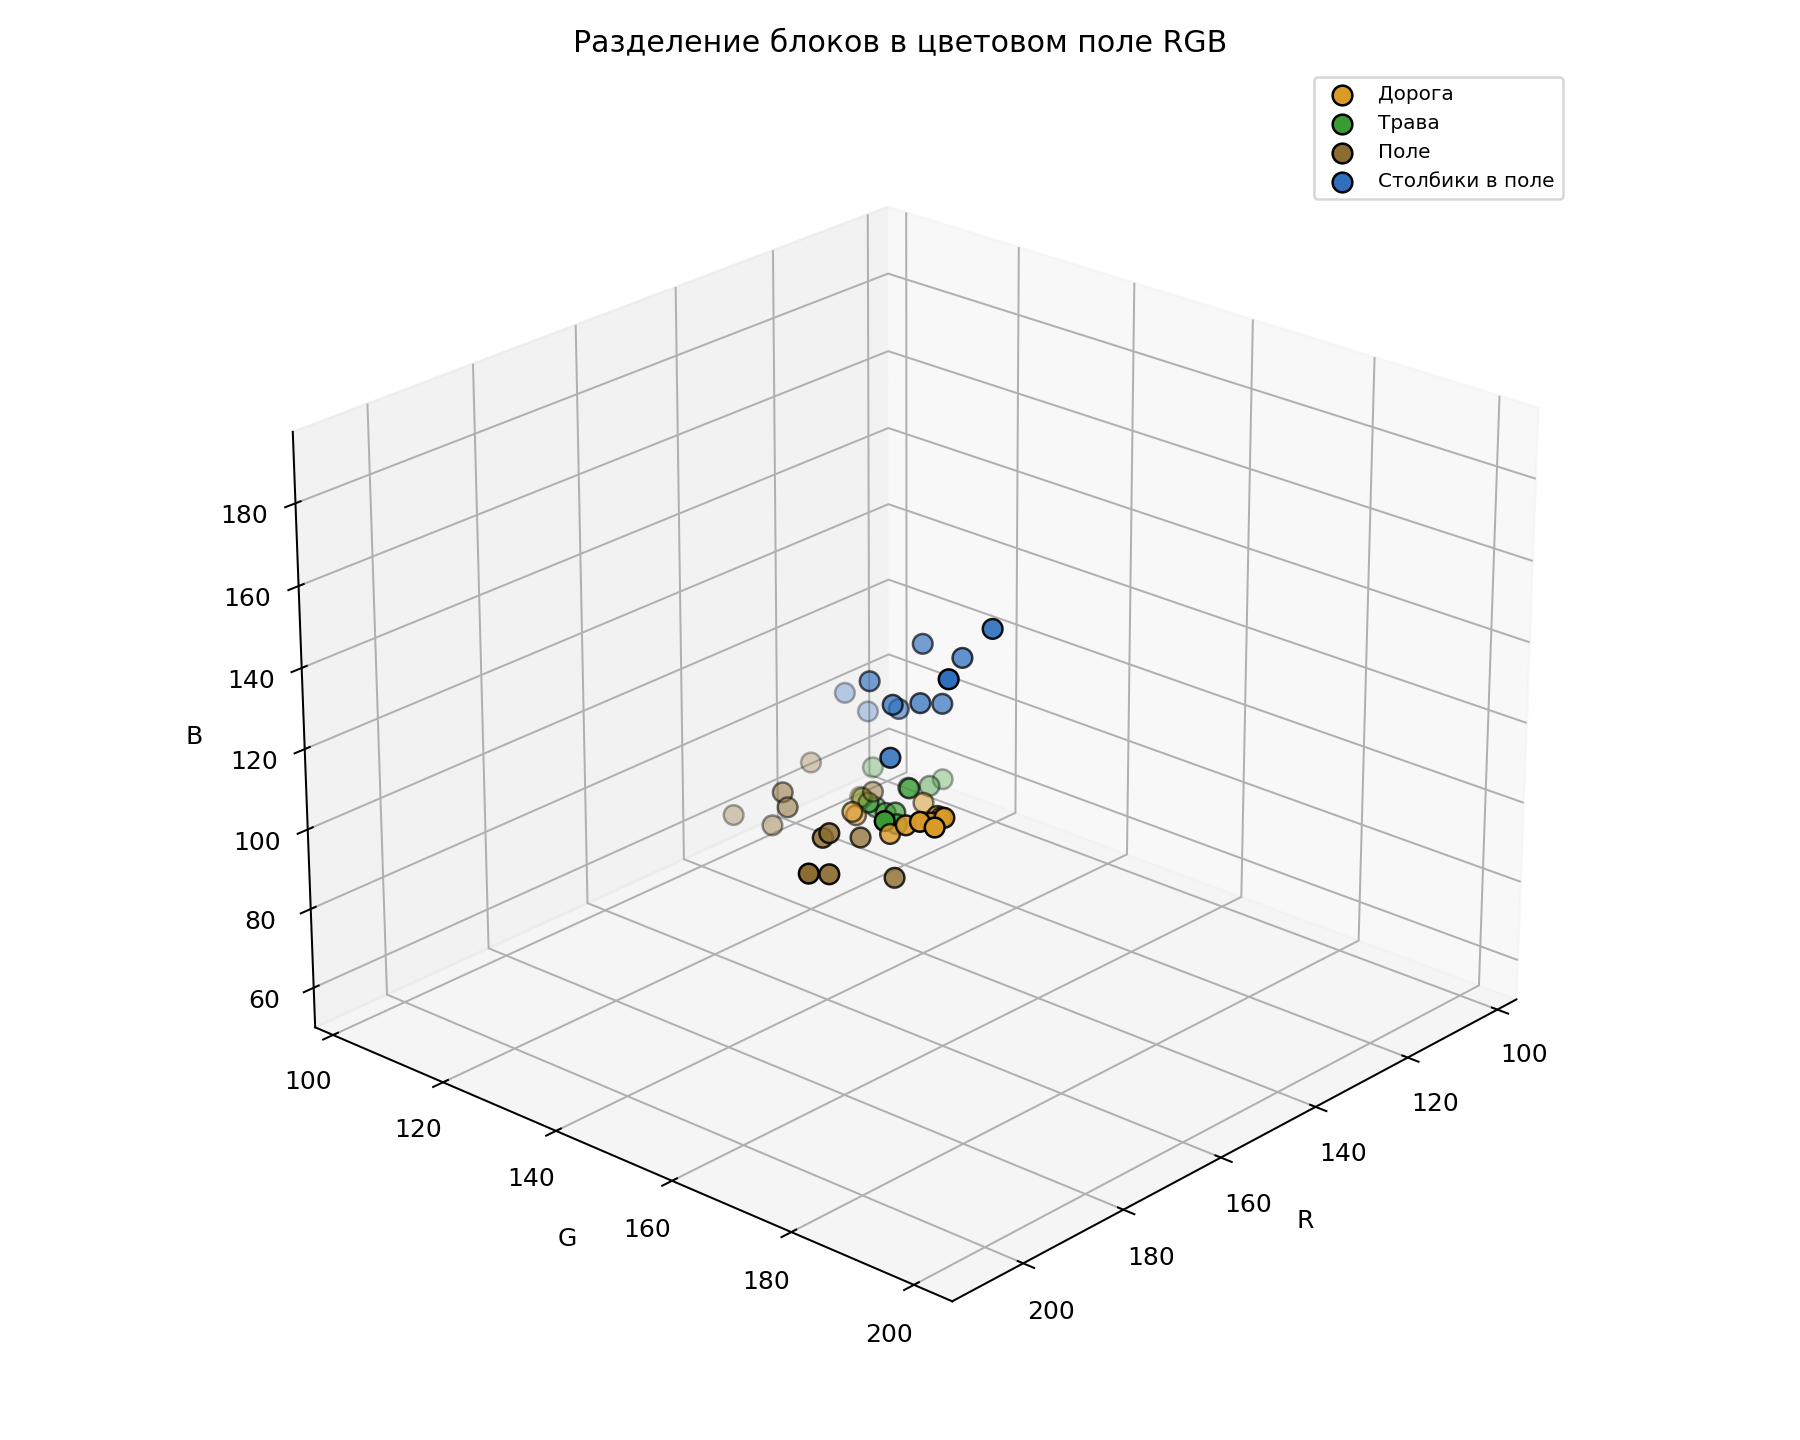
\includegraphics[width=\linewidth]{img/rgb_color_field_3d.png}
\caption{RGB, 3D}
\end{subfigure}\hfill
\begin{subfigure}[b]{0.49\textwidth}\centering
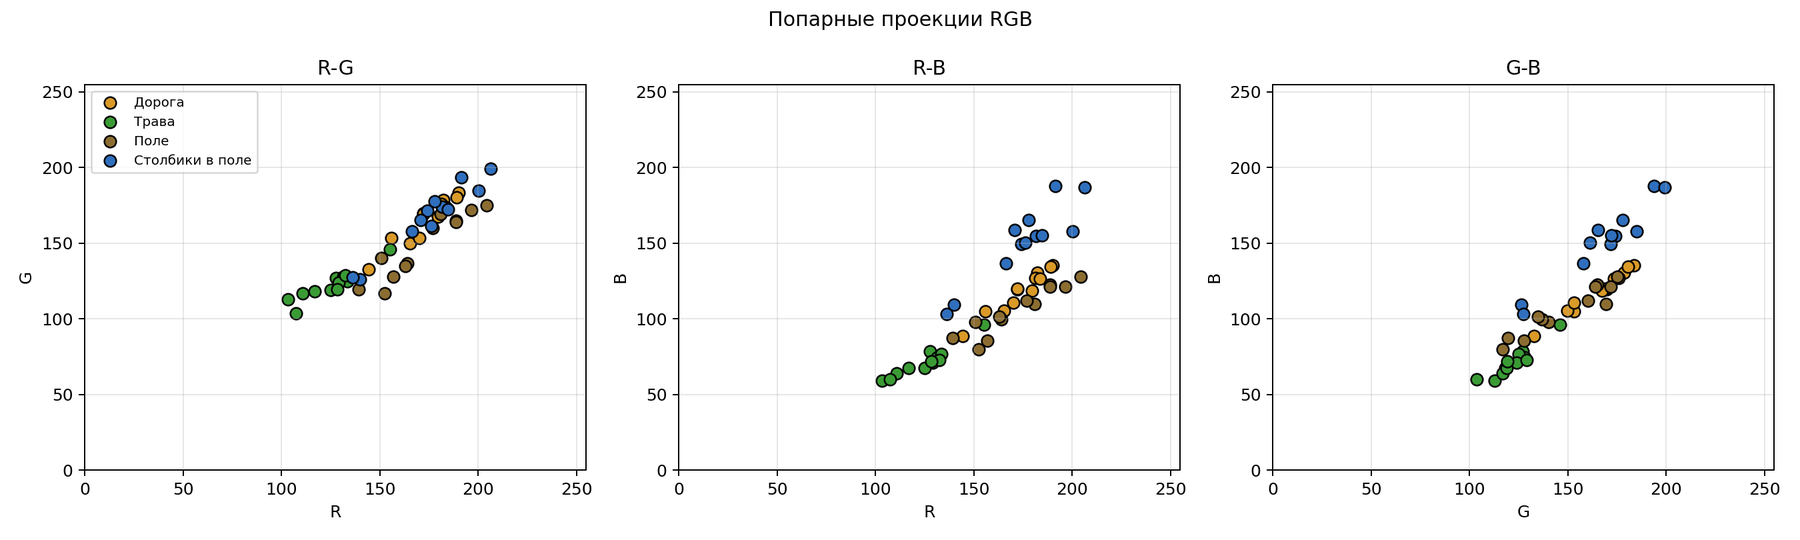
\includegraphics[width=\linewidth]{img/rgb_pairwise_scatter.png}
\caption{Попарные проекции}
\end{subfigure}
\caption{Разделение выбранных блоков в цветовом поле RGB}
\end{figure}

\section*{Применённые преобразования (меню Image)}
При изменении порядка следования каналов форма распределений отдельных каналов сохраняется, но значения переходят в другие оси. Серый канал меняется, потому что он вычисляется с разными весами для Red, Green и Blue.

\begin{figure}[H]\centering
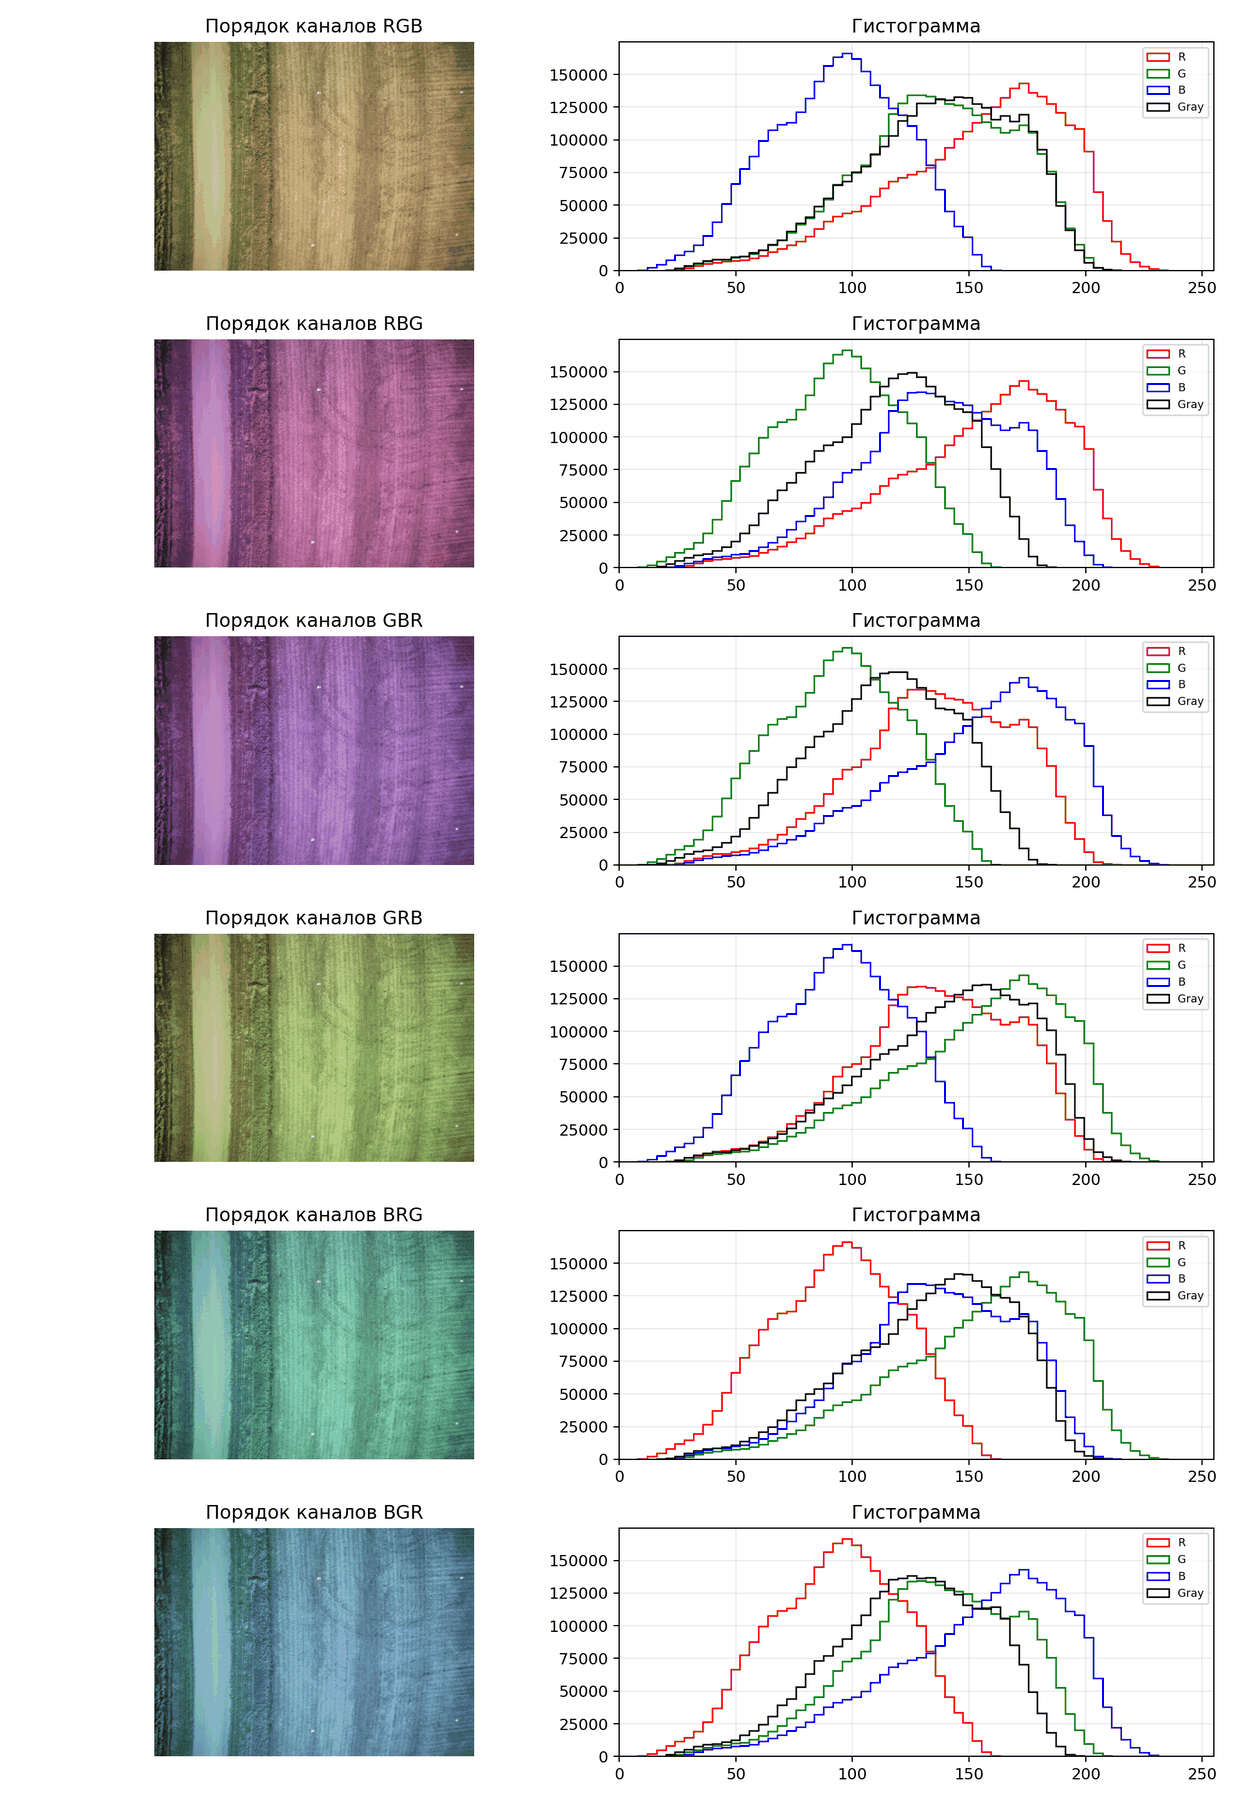
\includegraphics[width=0.92\textwidth]{img/task_2/swap_colors_histograms.png}
\caption{Перестановка каналов RGB и соответствующие гистограммы}
\end{figure}

При уменьшении контрастности до 50\% гистограммы сжимаются к средним значениям, поэтому различение поверхностей становится хуже. При увеличении контрастности до 150\% распределения растягиваются, различие между классами становится заметнее, но часть деталей в самых светлых и темных областях может теряться.

\begin{figure}[H]\centering
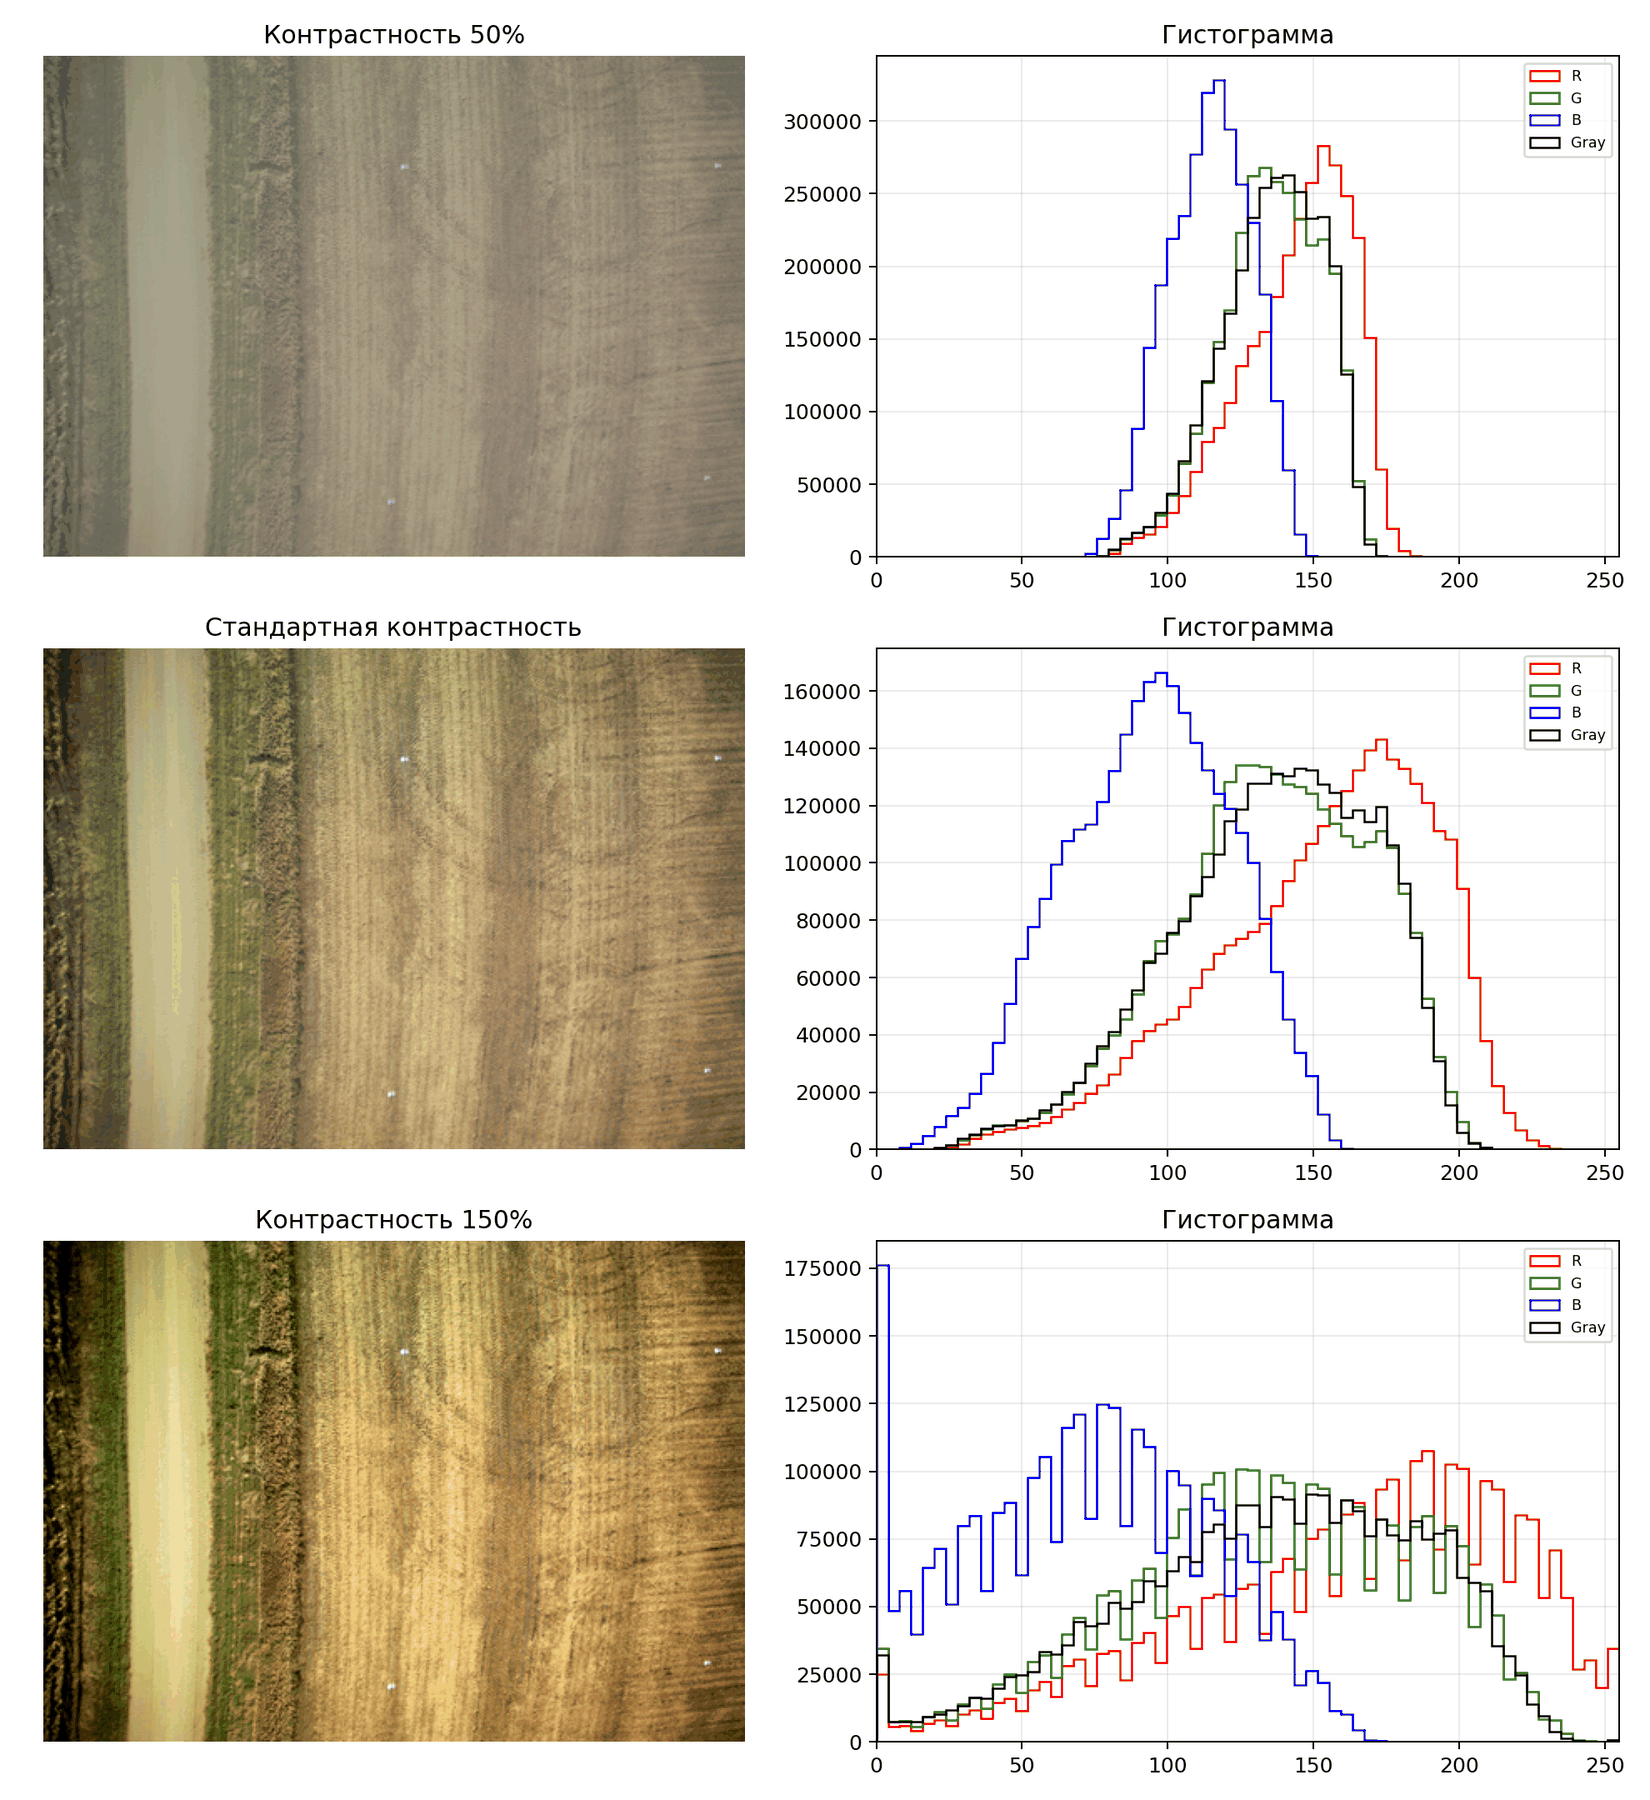
\includegraphics[width=0.92\textwidth]{img/task_2/contrast_histograms.png}
\caption{Гистограммы при уменьшенной, стандартной и увеличенной контрастности}
\end{figure}

\begin{figure}[H]
\centering
\begin{subfigure}[b]{0.49\textwidth}\centering
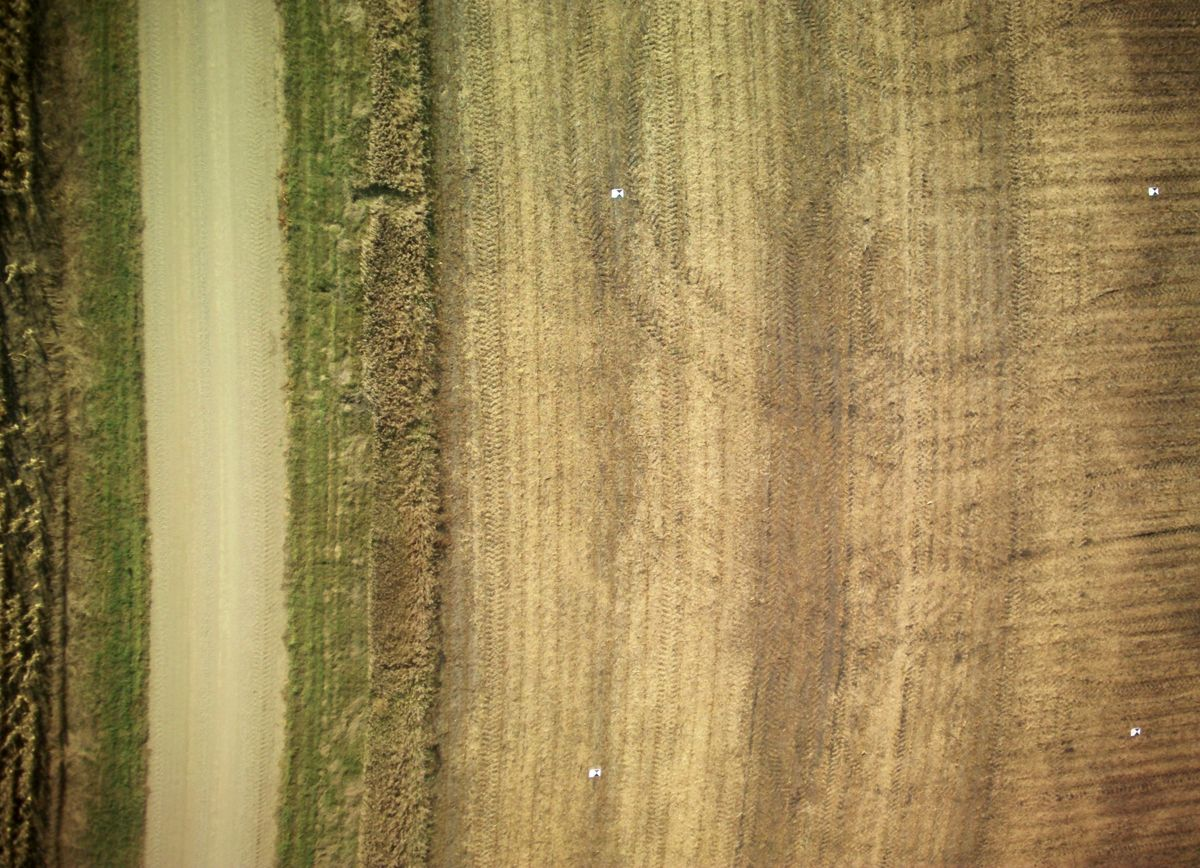
\includegraphics[width=\linewidth]{img/task_2/auto_adjust_col.jpg}
\caption{Auto adjust colors}
\end{subfigure}\hfill
\begin{subfigure}[b]{0.49\textwidth}\centering
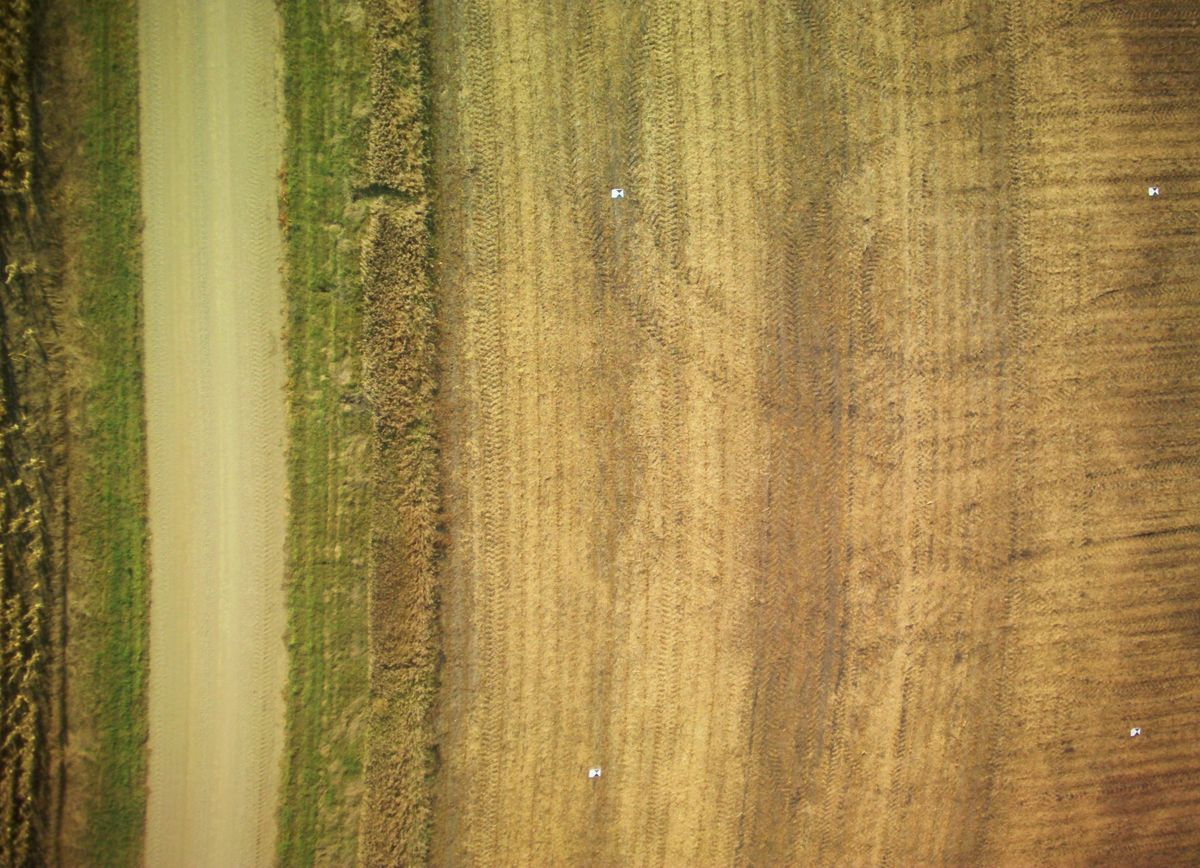
\includegraphics[width=\linewidth]{img/task_2/col_corect.jpg}
\caption{Color correction}
\end{subfigure}\\[0.3cm]
\begin{subfigure}[b]{0.49\textwidth}\centering
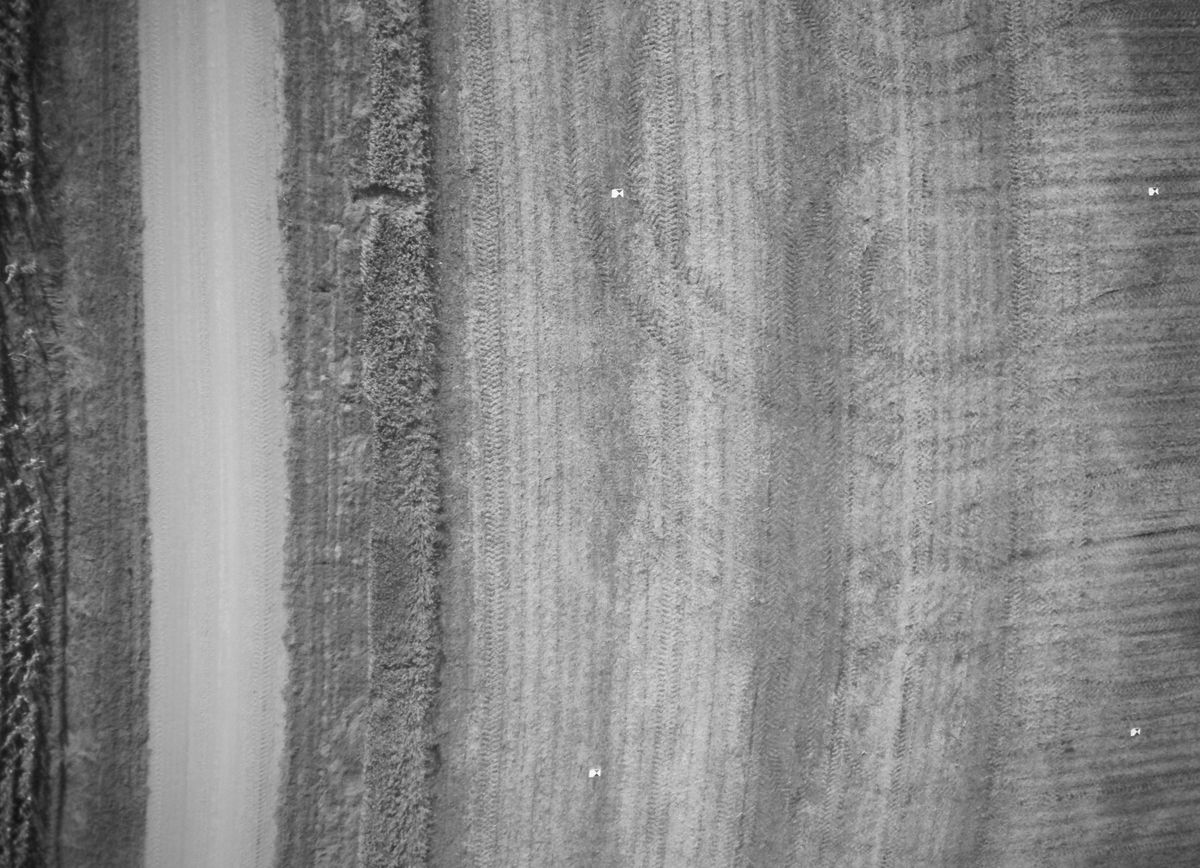
\includegraphics[width=\linewidth]{img/task_2/conv_to_grey_scale.jpg}
\caption{Convert to greyscale}
\end{subfigure}\hfill
\begin{subfigure}[b]{0.49\textwidth}\centering
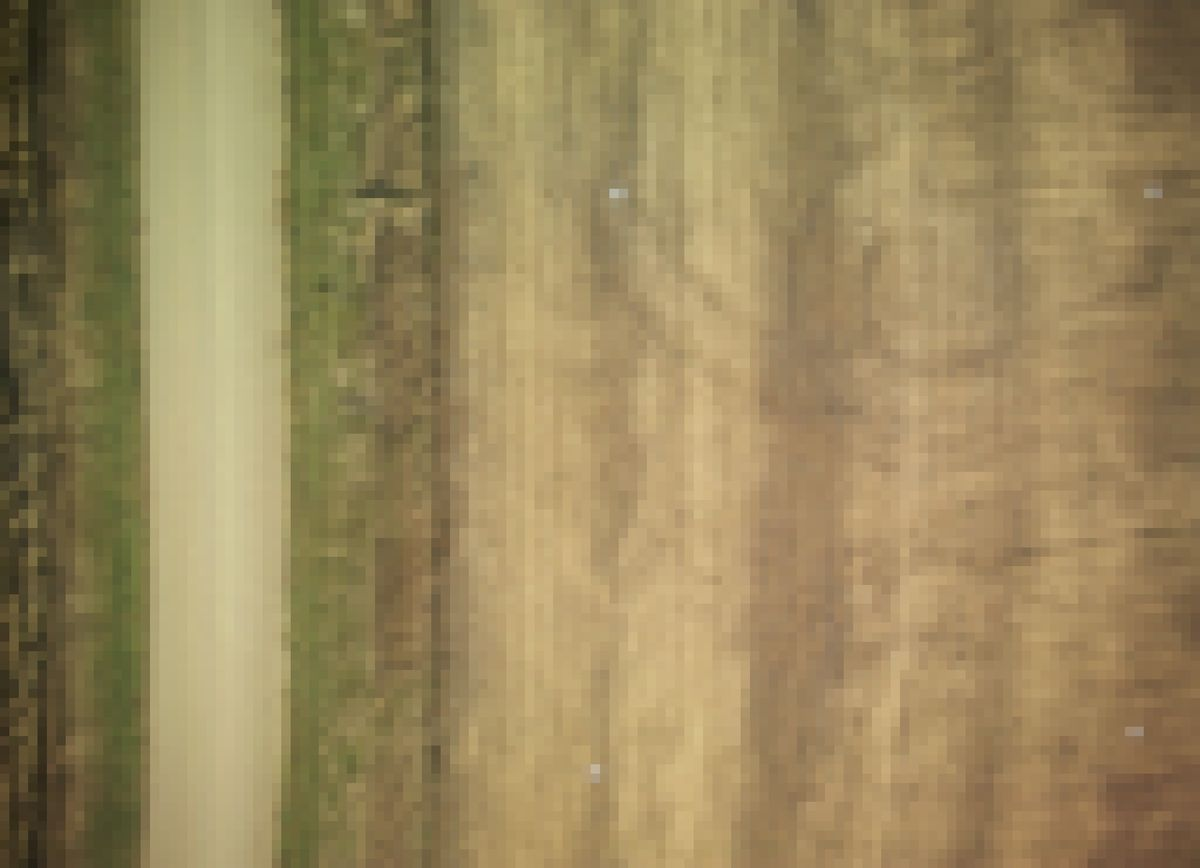
\includegraphics[width=\linewidth]{img/task_2/effect_pixelize.jpg}
\caption{Pixelize}
\end{subfigure}
\caption{Дополнительные преобразования}
\end{figure}

\section*{Выводы}
В работе выделены четыре класса: дорога, трава, поле и столбики в поле. Для каждого класса использовано по 12 блоков размером 18x18 пикселей. Трава лучше всего отделяется по низкому значению синего канала, столбики - по повышенной яркости и синему каналу, а дорога и поле частично пересекаются по Red, но различаются по Green, Blue и дисперсии. Перестановка каналов изменяет визуальное восприятие изображения и распределение серого канала, а увеличение контрастности повышает различимость гистограмм по сравнению с уменьшенной контрастностью.

\end{document}
